%==============================================================
This chapter describes the detailed operation of the 4004 CPU, its specific interactions with ROM and RAM, and the specifications of its Instruction Set Archtecture.
%==============================================================
\section{4004 CPU Programmer's Model}
Figure \ref{fig:CPUPROGRAMMERSMODEL} illustrates the programmer's model of the 4004 CPU. Each resource is described below.

\begin{enumerate}
  \item \textbf{Accumulator (ACC):} A 4-bit wide register used for arithmetic operations such as addition and subtraction, as well as for temporary data storage during ROM/RAM access.

  \item \textbf{Carry Bit (CY):} Used for carry in/out during 4-bit addition and borrow in/out during subtraction. It is also utilized in rotate instructions and can serve as a condition flag for branching instructions.

  \item \textbf{Index Register Group (R0--R15, R0P--R7P):} The CPU includes 16 x 4-bit index registers (R0 through R15). Even-numbered registers R[2n] serve as the upper 4 bits, and odd-numbered registers R[2n+1] serve as the lower 4 bits of 8-bit composite registers called index register pairs (RnP). For example, R0P consists of R0 (upper 4 bits) and R1 (lower 4 bits), while R4P comprises R8 and R9. These registers are used to store temporary data during computations or to hold partial address data for ROM/RAM access.

  \item \textbf{Designate Command Line Register (DCL):} A 3-bit register used to determine how the RAM control signals $\overline{\text{CM-RAM0}}$ through $\overline{\text{CM-RAM3}}$ are generated. It is set by the DCL instruction and reset to \texttt{000}. Details on the correspondence between DCL values and $\overline{\text{CM-RAM}}$ signals are discussed later.

  \item \textbf{Stack (Program Address Registers):} The CPU provides a 4-level stack structure composed of 12-bit program address registers. A virtual 2-bit stack pointer (SP) indicates which stack level is active. The program address register pointed to by SP functions as the program counter (PC). Upon executing the subroutine call instruction \texttt{JMS}, SP increments and a new program address register becomes the PC, storing the branch destination. The previous PC register holds the return address. When the return-from-subroutine instruction \texttt{BBL} is executed, SP decrements, and the return address becomes the new PC, allowing the routine to resume.
\end{enumerate}

%----------------------------------
\begin{figure}[h]
    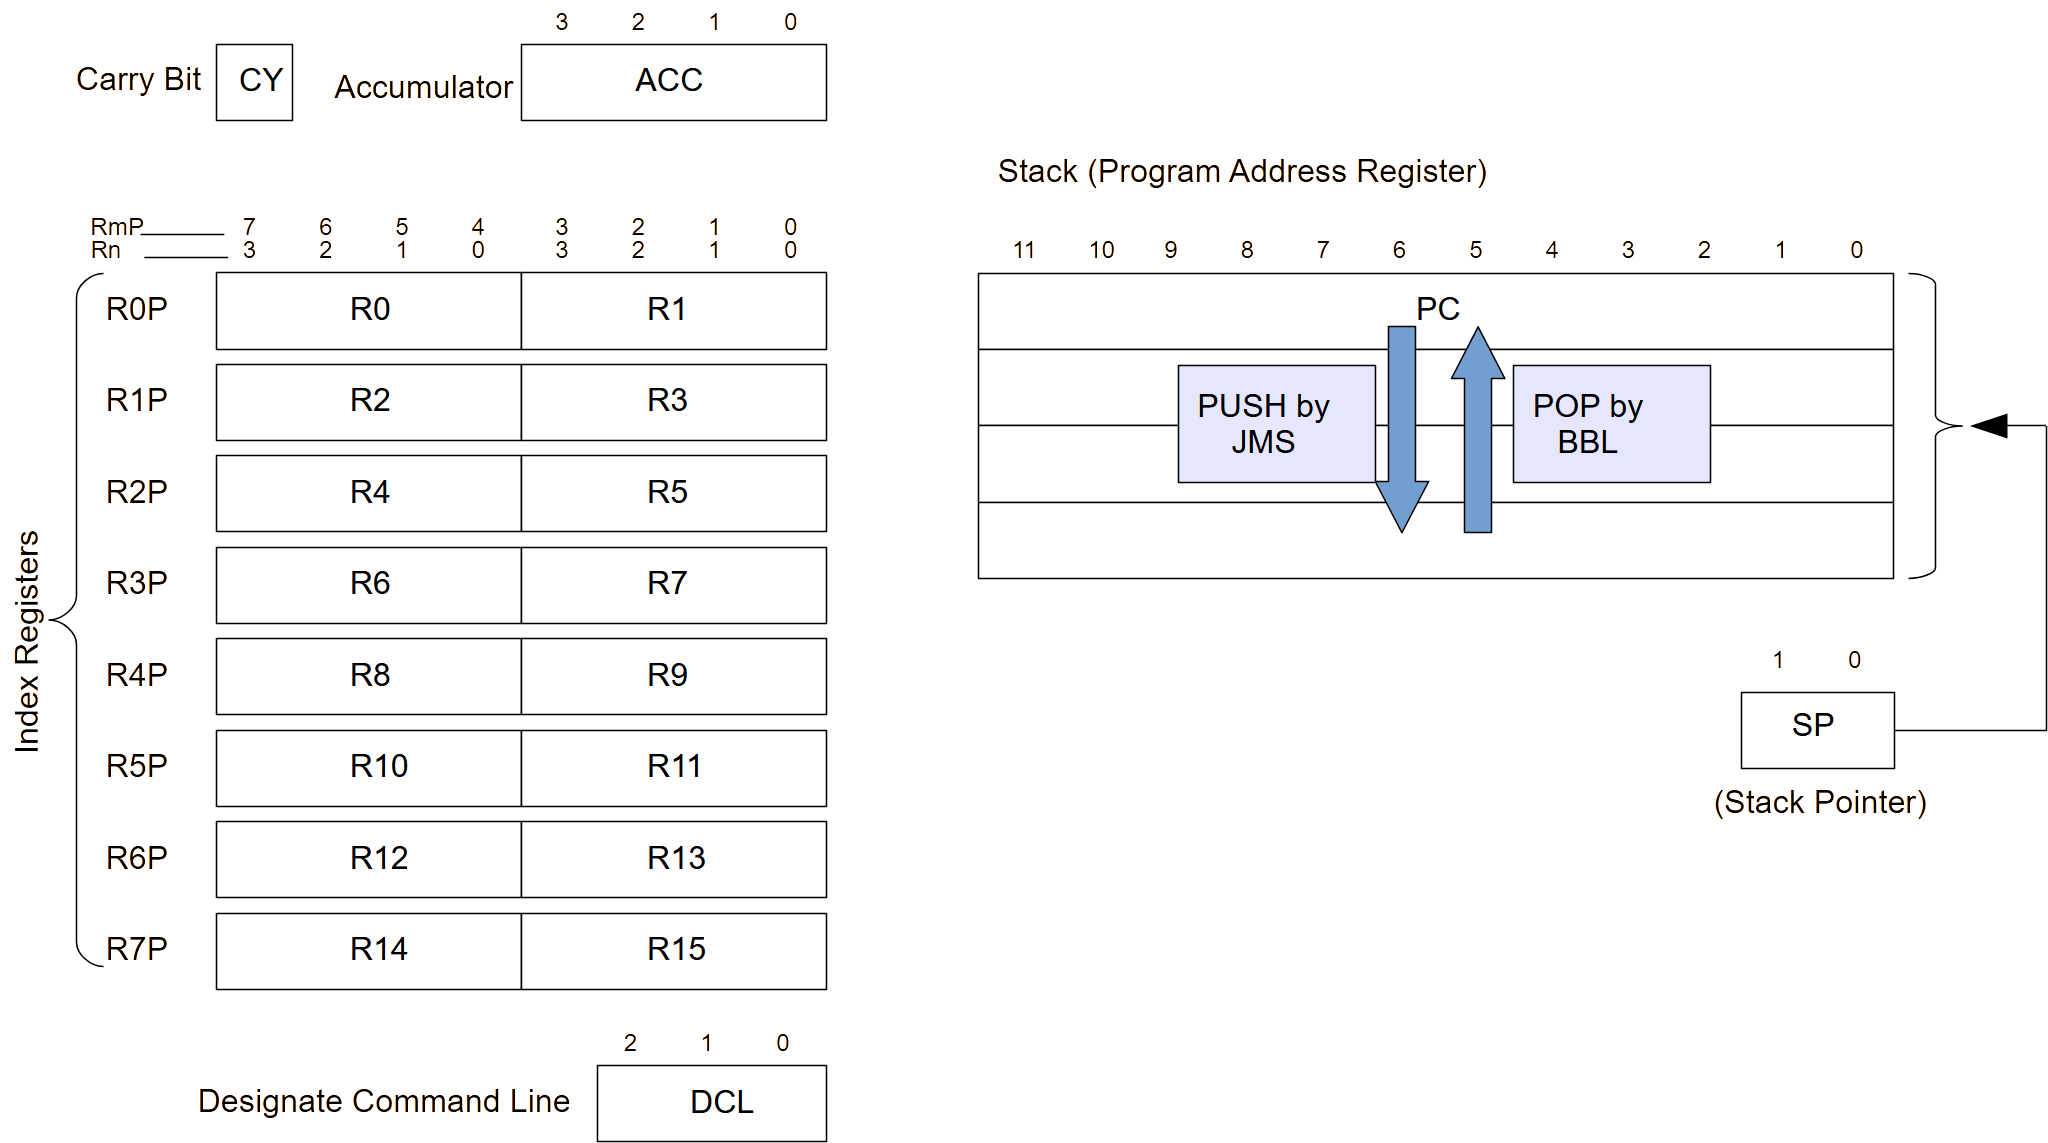
\includegraphics[width=0.75\columnwidth]{./Figure/CPUProgrammersModel.png}
    \caption{4004 CPU Programmers Model}
    \label{fig:CPUPROGRAMMERSMODEL}
\end{figure}
%----------------------------------

%==============================================================
\section{Instruction Timing of the CPU}
Figure \ref{fig:CPUINSTRUCTIONTIMING} illustrates the timing of CPU instructions. The CPU operates on an 8 clock instruction cycle, which consists of the following eight states:

\begin{enumerate}
  \item \textbf{State A1:} Outputs the lower 4 bits of the ROM address, PC[3:0], onto the data bus.
  
  \item \textbf{State A2:} Outputs the middle 4 bits of the ROM address, PC[7:4], onto the data bus.

  \item \textbf{State A3:} Outputs the upper 4 bits of the ROM address, PC[11:8], onto the data bus. Simultaneously, asserts $\overline{\text{CM-ROM}}$ and the $\overline{\text{CM-RAMx}}$ signal selected via the DCL register.

  \item \textbf{State M1:} Inputs the upper 4 bits of data (OPR) from ROM through the data bus.

  \item \textbf{State M2:} Inputs the lower 4 bits of data (OPA) from ROM through the data bus. If the previously read OPR is a data access instruction, $\overline{\text{CM-ROM}}$ and the $\overline{\text{CM-RAMx}}$ signal selected via DCL are asserted to inform ROM/RAM of the access type.

  \item \textbf{State X1:} Instruction execution state for internal processing.

  \item \textbf{State X2:} Another instruction execution state, which may involve internal processing or outputting the upper 4 bits of a ROM/RAM (I/O ports or memory) address onto the data bus. It may also handle reading from or writing to ROM/RAM via the data bus. If outputting address bits, $\overline{\text{CM-ROM}}$ and DCL-selected $\overline{\text{CM-RAMx}}$ are asserted.

  \item \textbf{State X3:} Instruction execution state that may perform internal processing or output the lower 4 bits of a ROM/RAM address onto the data bus.
\end{enumerate}

\subsection{Synchronization of CPU, ROM, and RAM}
During State X3, the CPU asserts the $\overline{\text{SYNC}}$ signal to synchronize operations with ROM and RAM. All three units operate under a shared clock and proceed through their internal states in complete synchrony.

%----------------------------------
\begin{figure}[htbp]
    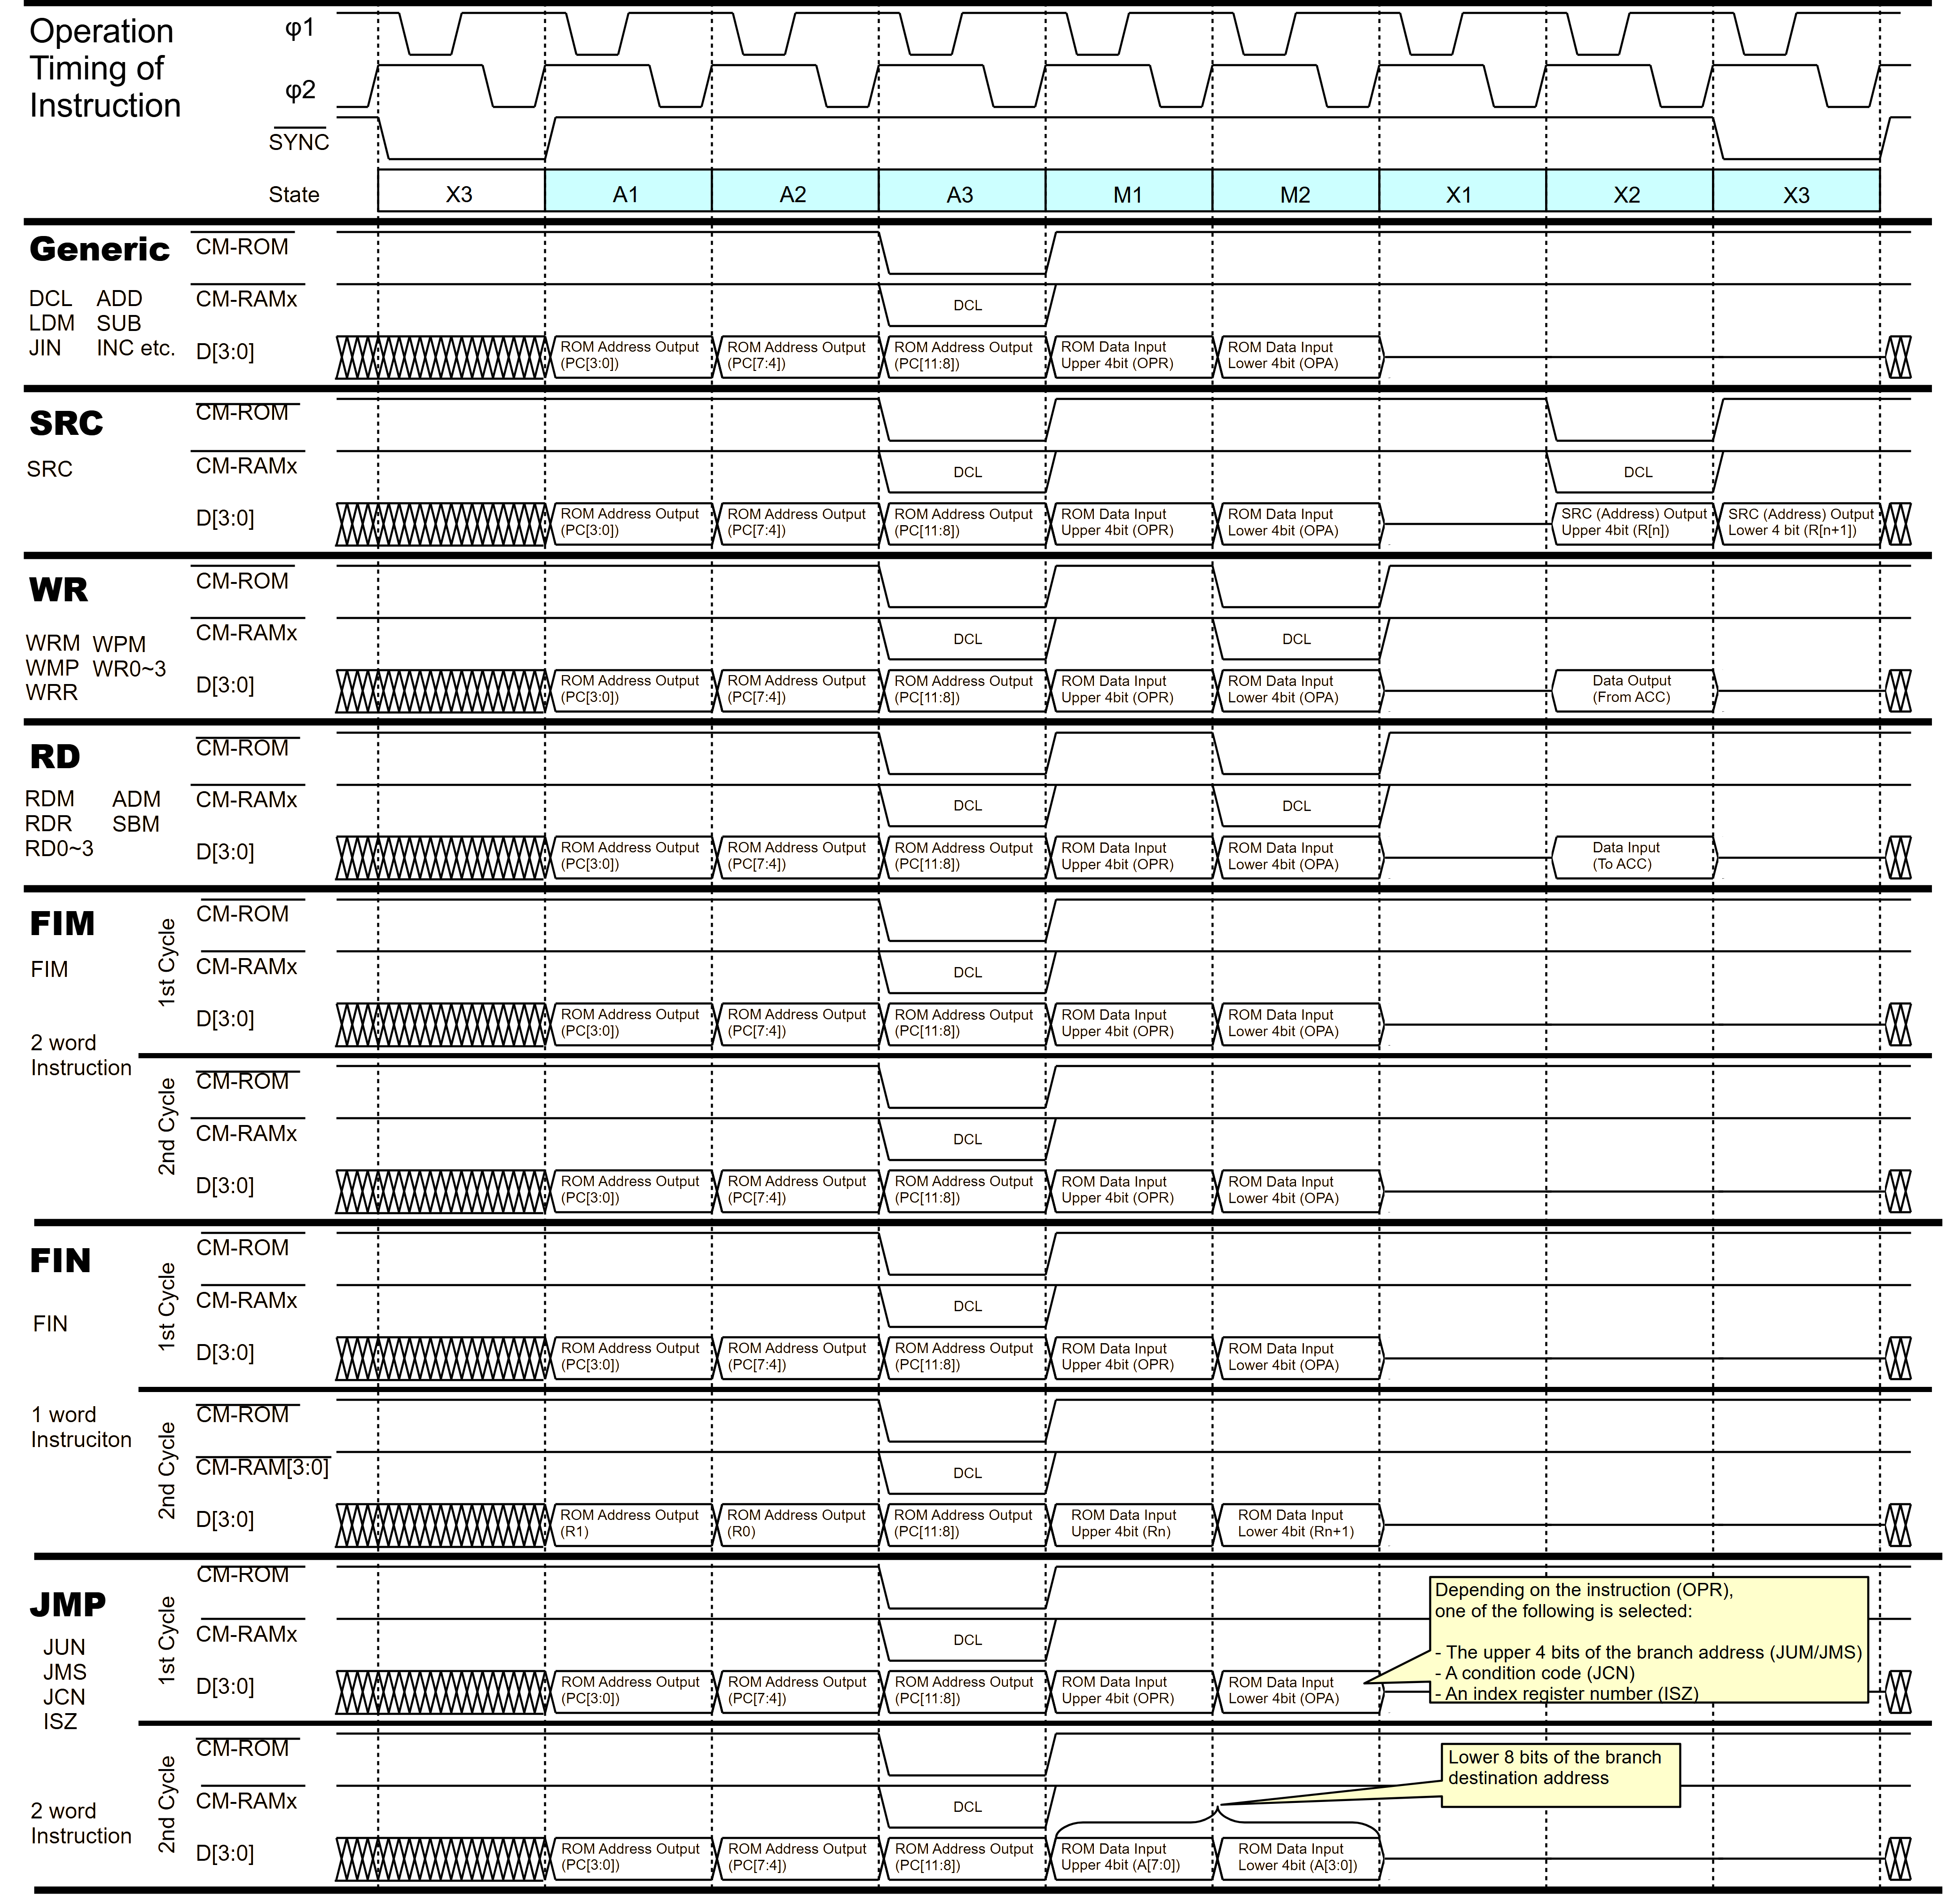
\includegraphics[width=1.0\columnwidth]{./Figure/CPUInstructionTiming.png}
    \caption{4004 CPU Instruction Timing}
    \label{fig:CPUINSTRUCTIONTIMING}
\end{figure}
%----------------------------------
%==============================================================
\section{Instruction Set Architecture and Opcode Tables}
Specifications and opcodes for each 4004 CPU instruction Set Architecture are presented in Tables \ref{tb:ISA1MACHINE1WORD} through \ref{tb:ISA4ACCUMULATOR}.

Table \ref{tb:ISA1MACHINE1WORD} contains single-word instructions (8 bits in length) categorized under the label ``Machine Instructions''. While ``machine instruction'' typically refers to any instruction written in machine language, here it appears to serve as a specific category. It is possible that this grouping includes commands that are neither related to data access nor the accumulator. Among these, the \texttt{FIN} instruction stands out: although it is a single-word instruction, it requires two instruction cycles to execute.

Table \ref{tb:ISA2MACHINE2WORD} lists the machine instructions that span two words (16 bits total).

Table \ref{tb:ISA3DATAACCESS} covers single-word data access instructions (8 bits). These involve reading from and writing to ROM I/O ports, RAM memory, and RAM output ports.

Table \ref{tb:ISA4ACCUMULATOR} includes single-word accumulator-related instructions (8 bits).

Each instruction's operational characteristics, data flow, and associated control signals are detailed in their respective tables.

%----------------------------------
\begin{table}[htbp]
    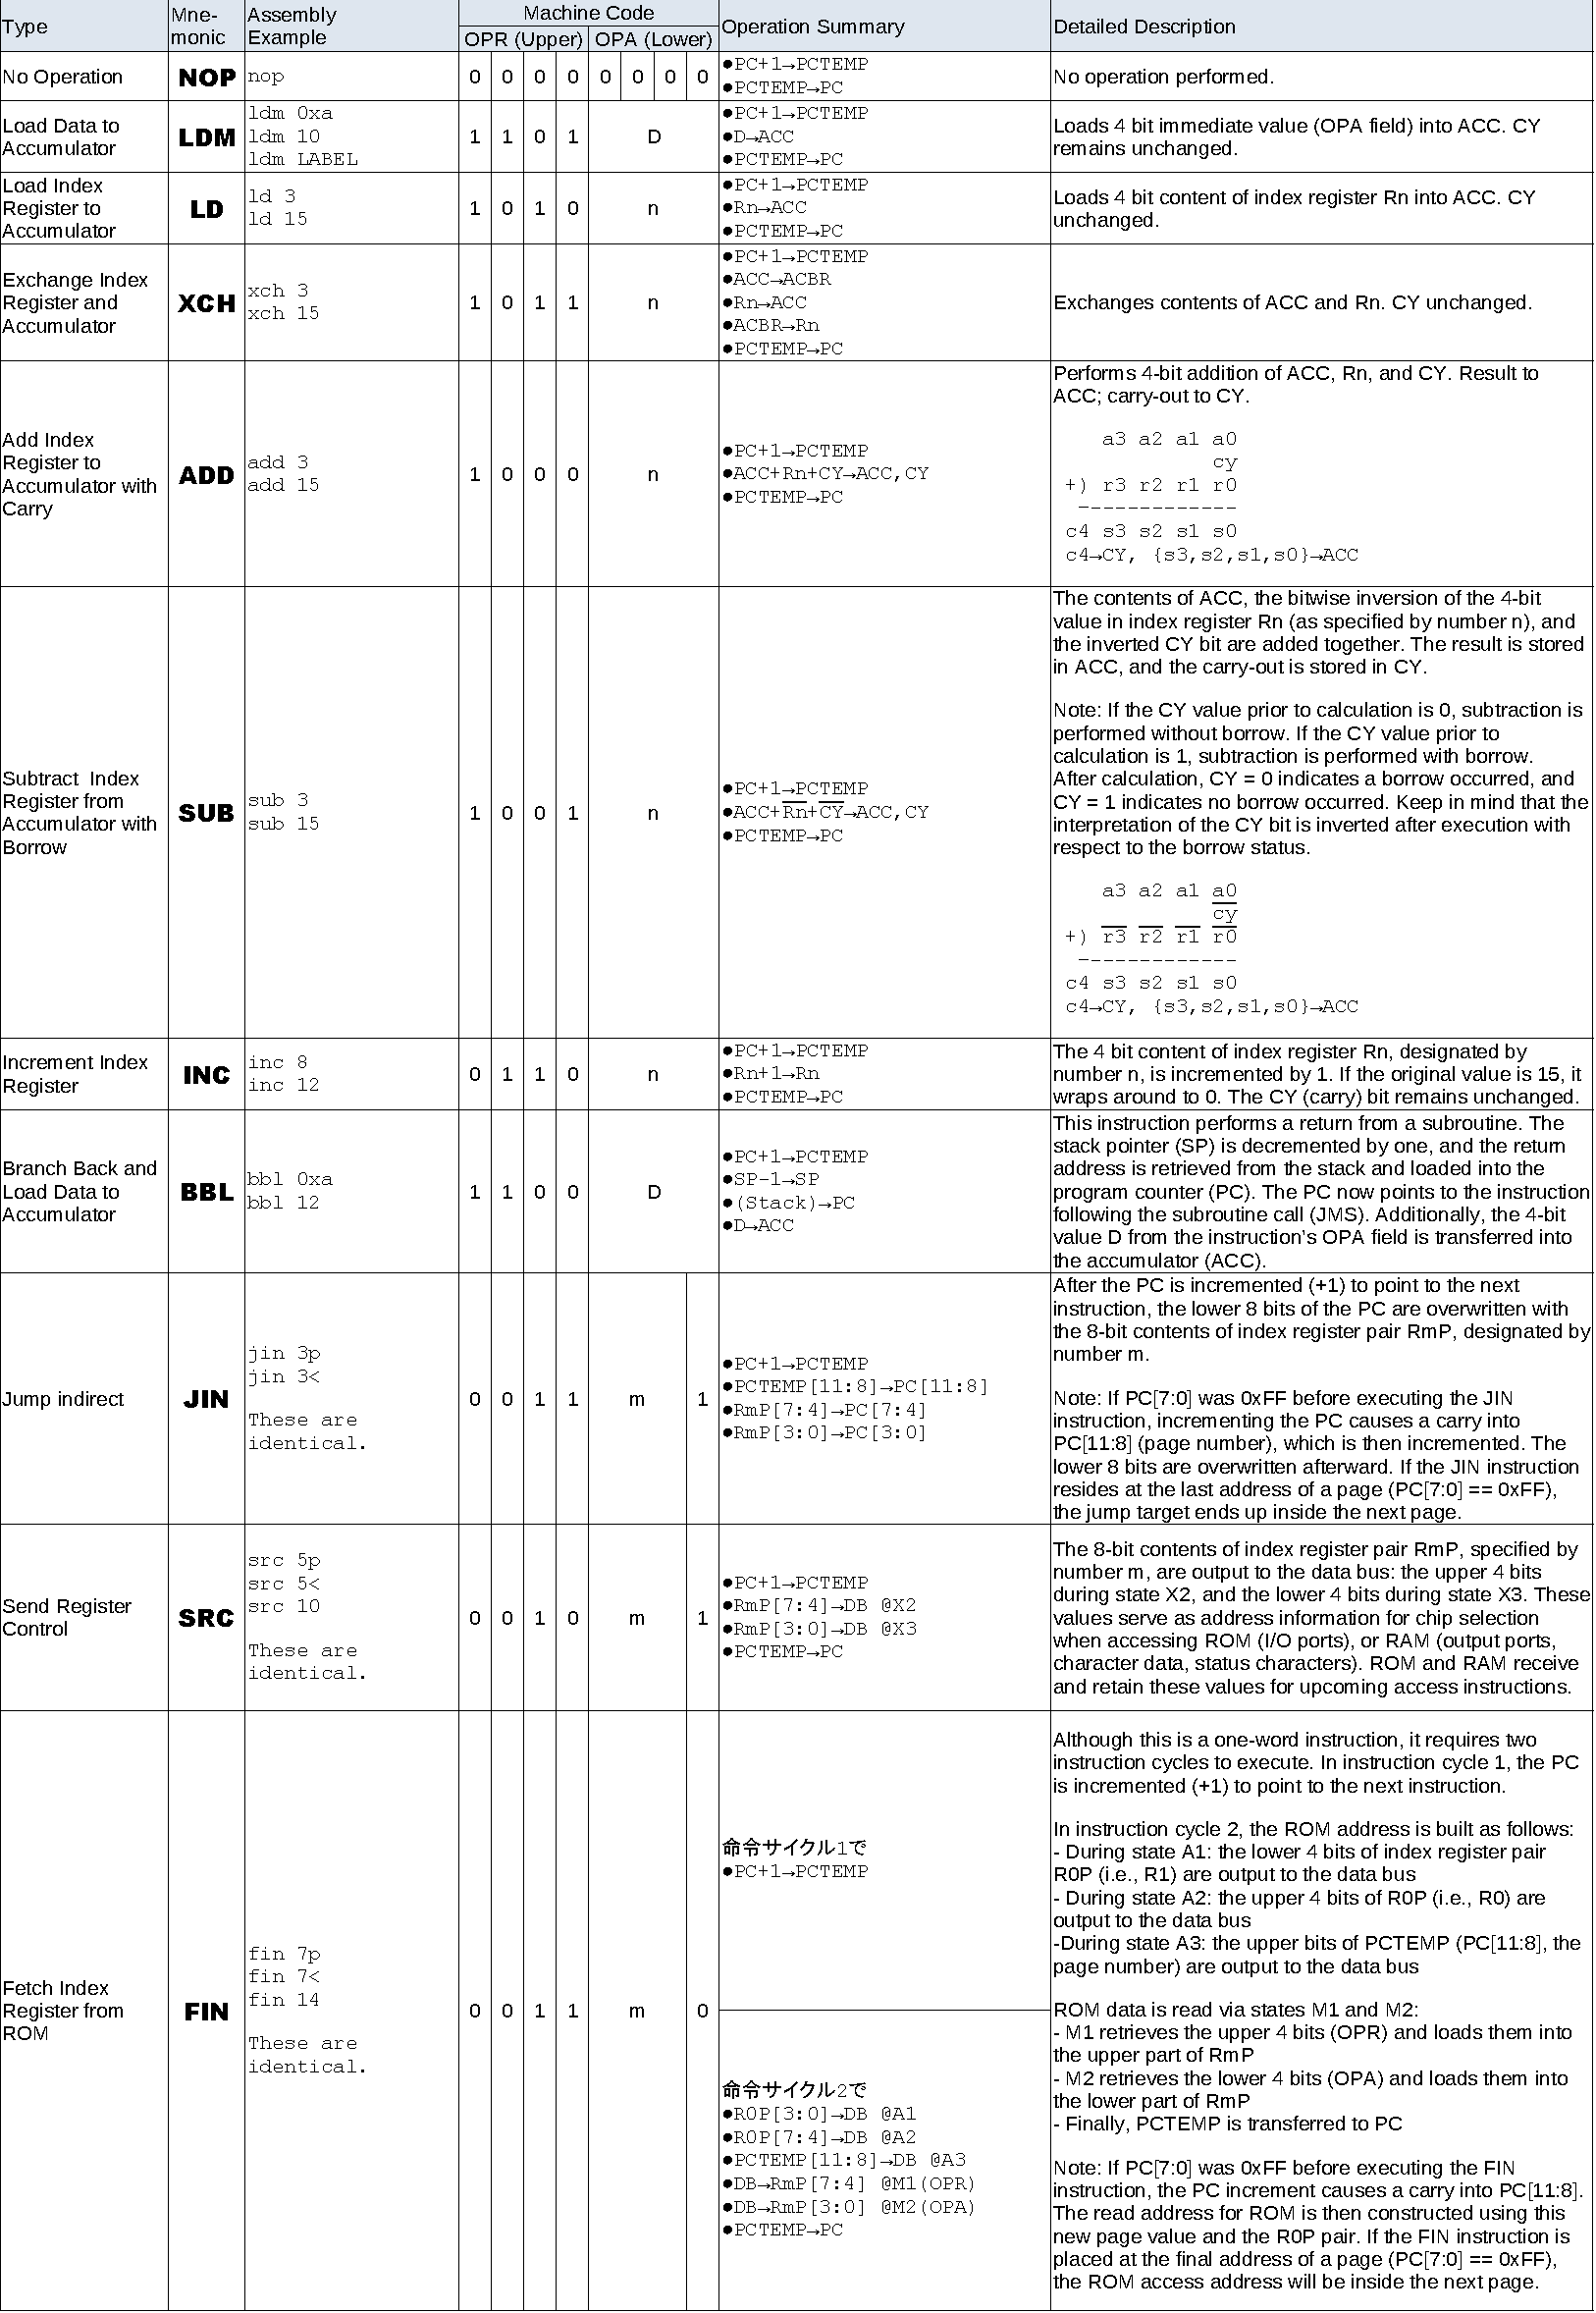
\includegraphics[width=1.00\columnwidth]{./Table/ISA(1)Machine(1word).pdf}
    \caption{CPU Instruciton Table (1) : Machine Instruction (1 word)}
    \label{tb:ISA1MACHINE1WORD}
\end{table}
%----------------------------------
%----------------------------------
\begin{table}[htbp]
    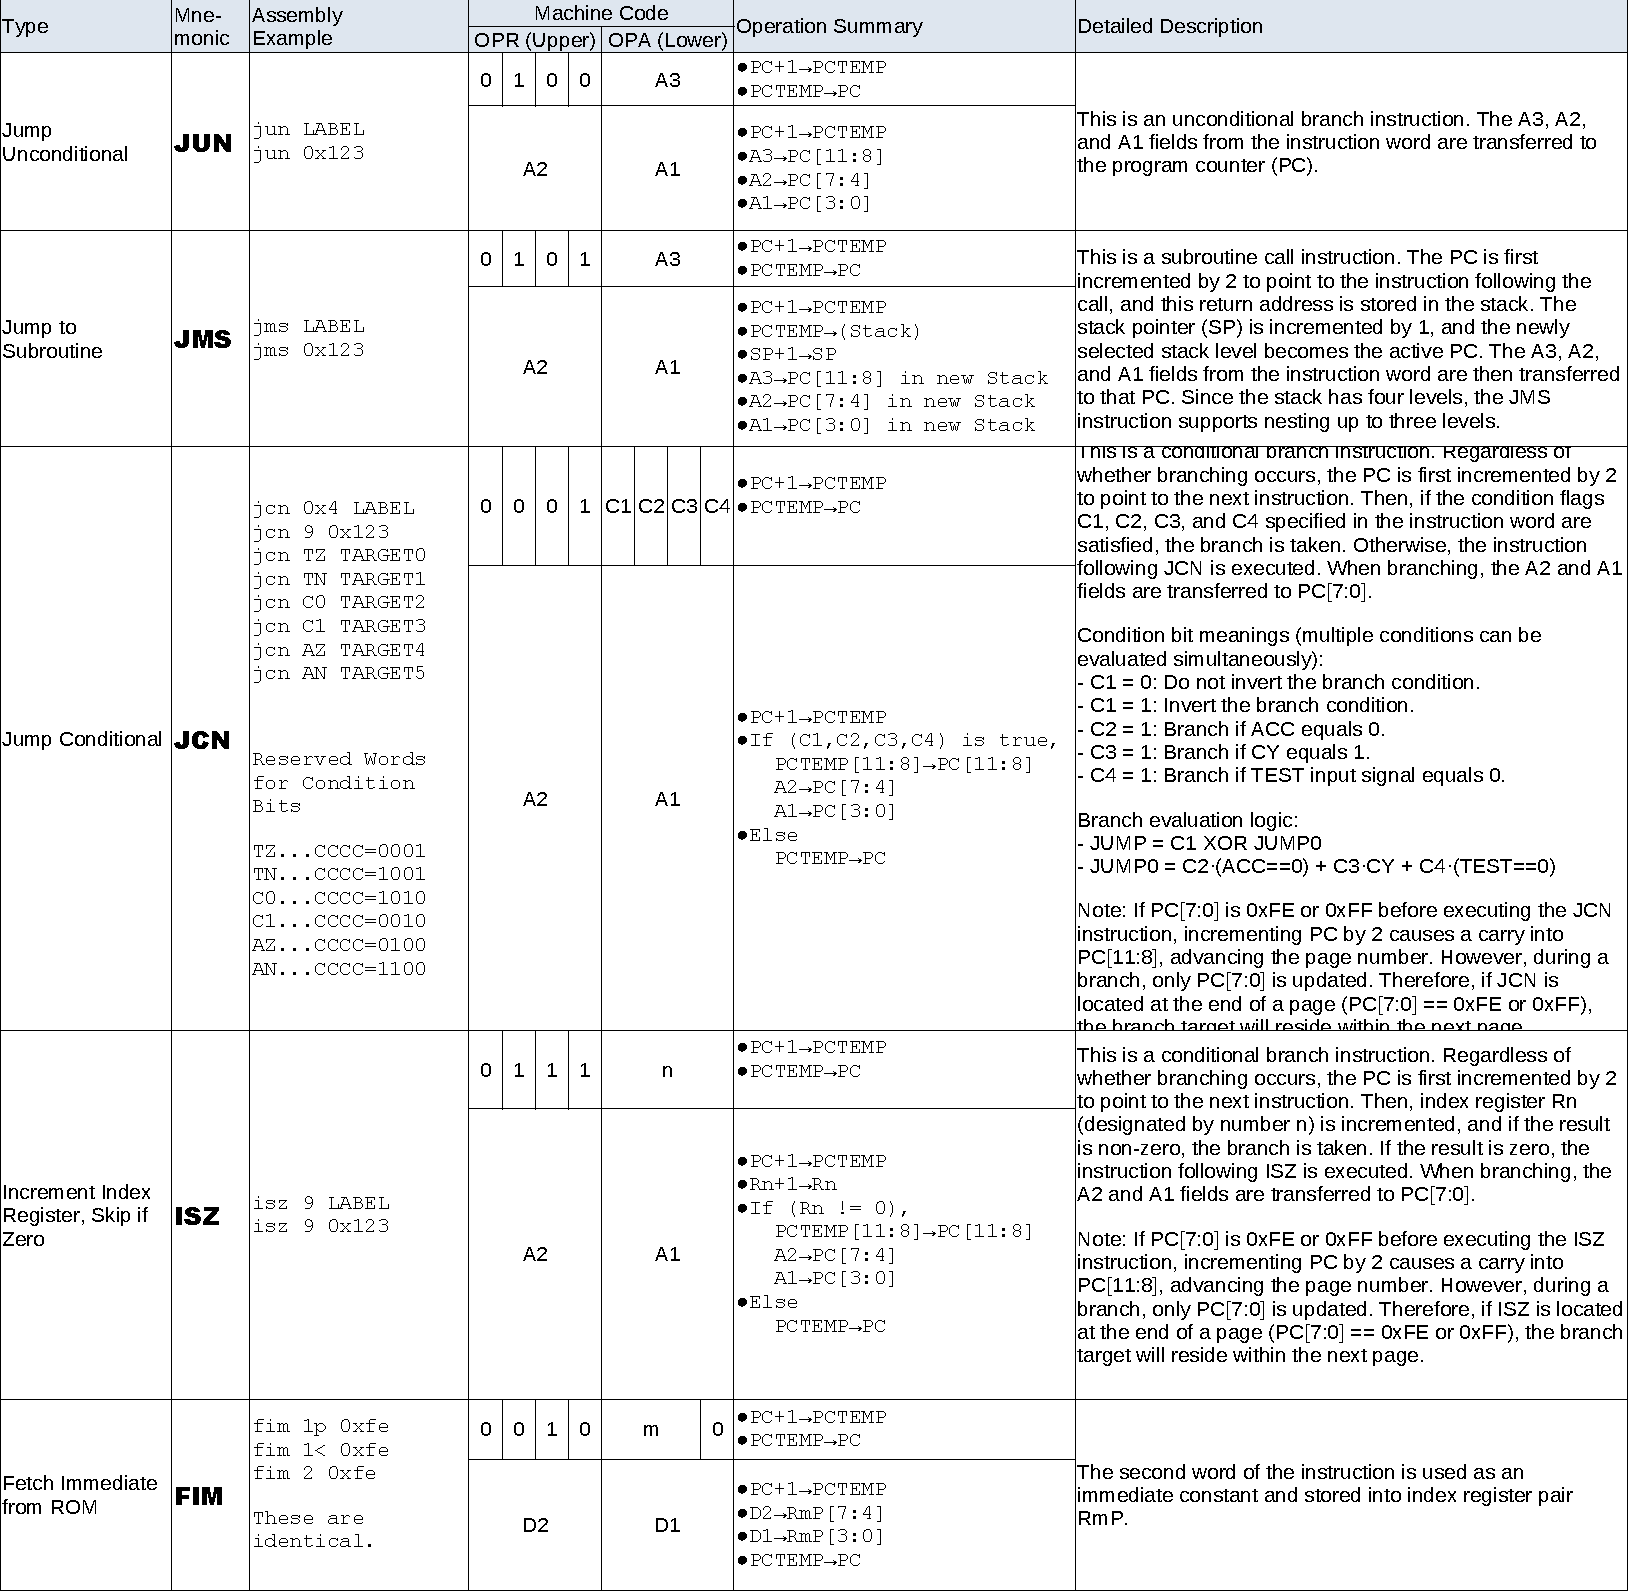
\includegraphics[width=1.00\columnwidth]{./Table/ISA(2)Machine(2word).pdf}
    \caption{CPU Instruciton Table (2) : Machine Instruction (2 word)}
    \label{tb:ISA2MACHINE2WORD}
\end{table}
%----------------------------------
%----------------------------------
\begin{table}[htbp]
    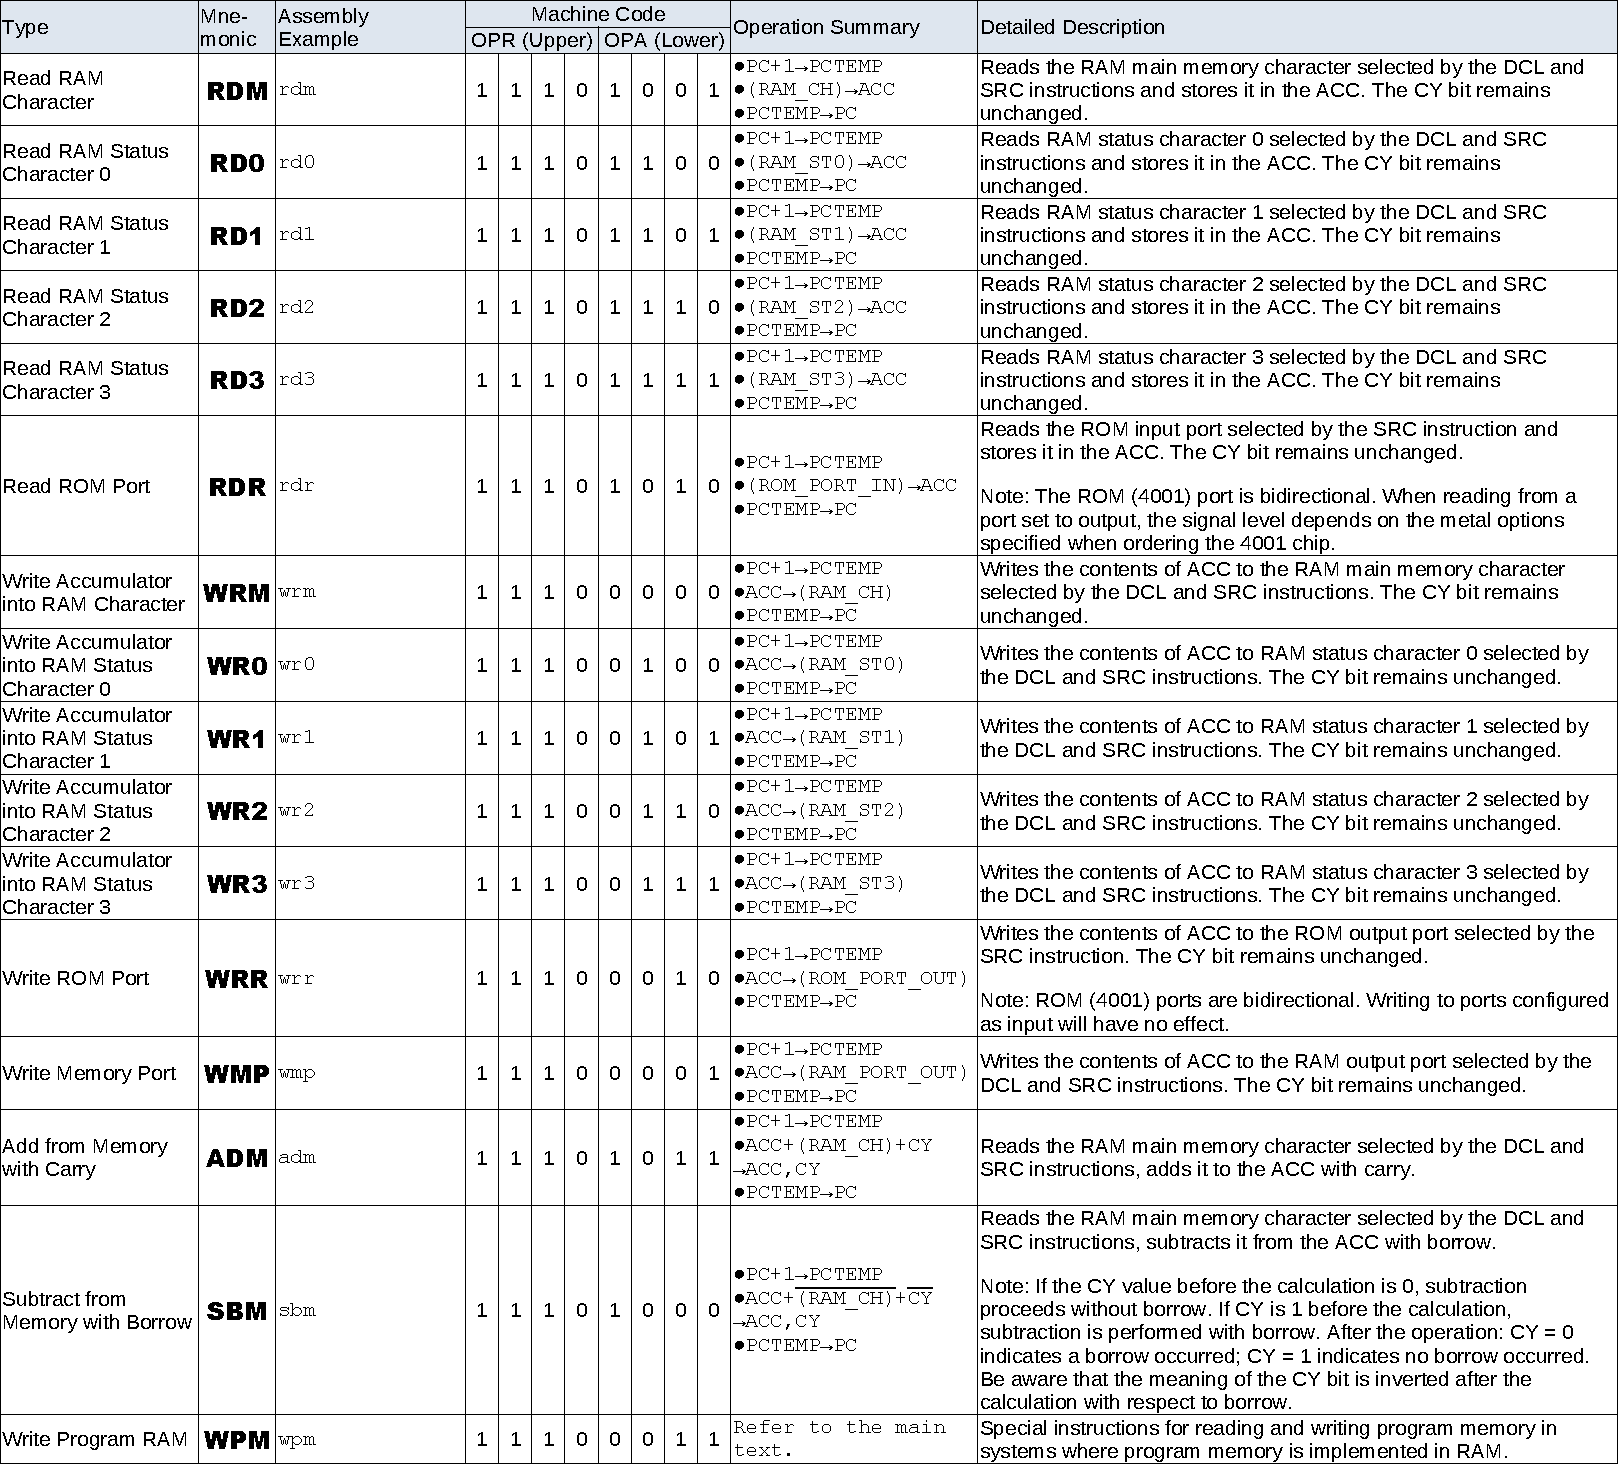
\includegraphics[width=1.00\columnwidth]{./Table/ISA(3)DataAccess.pdf}
    \caption{CPU Instruciton Table (3) : Data Access}
    \label{tb:ISA3DATAACCESS}
\end{table}
%----------------------------------
%----------------------------------
\begin{table}[htbp]
    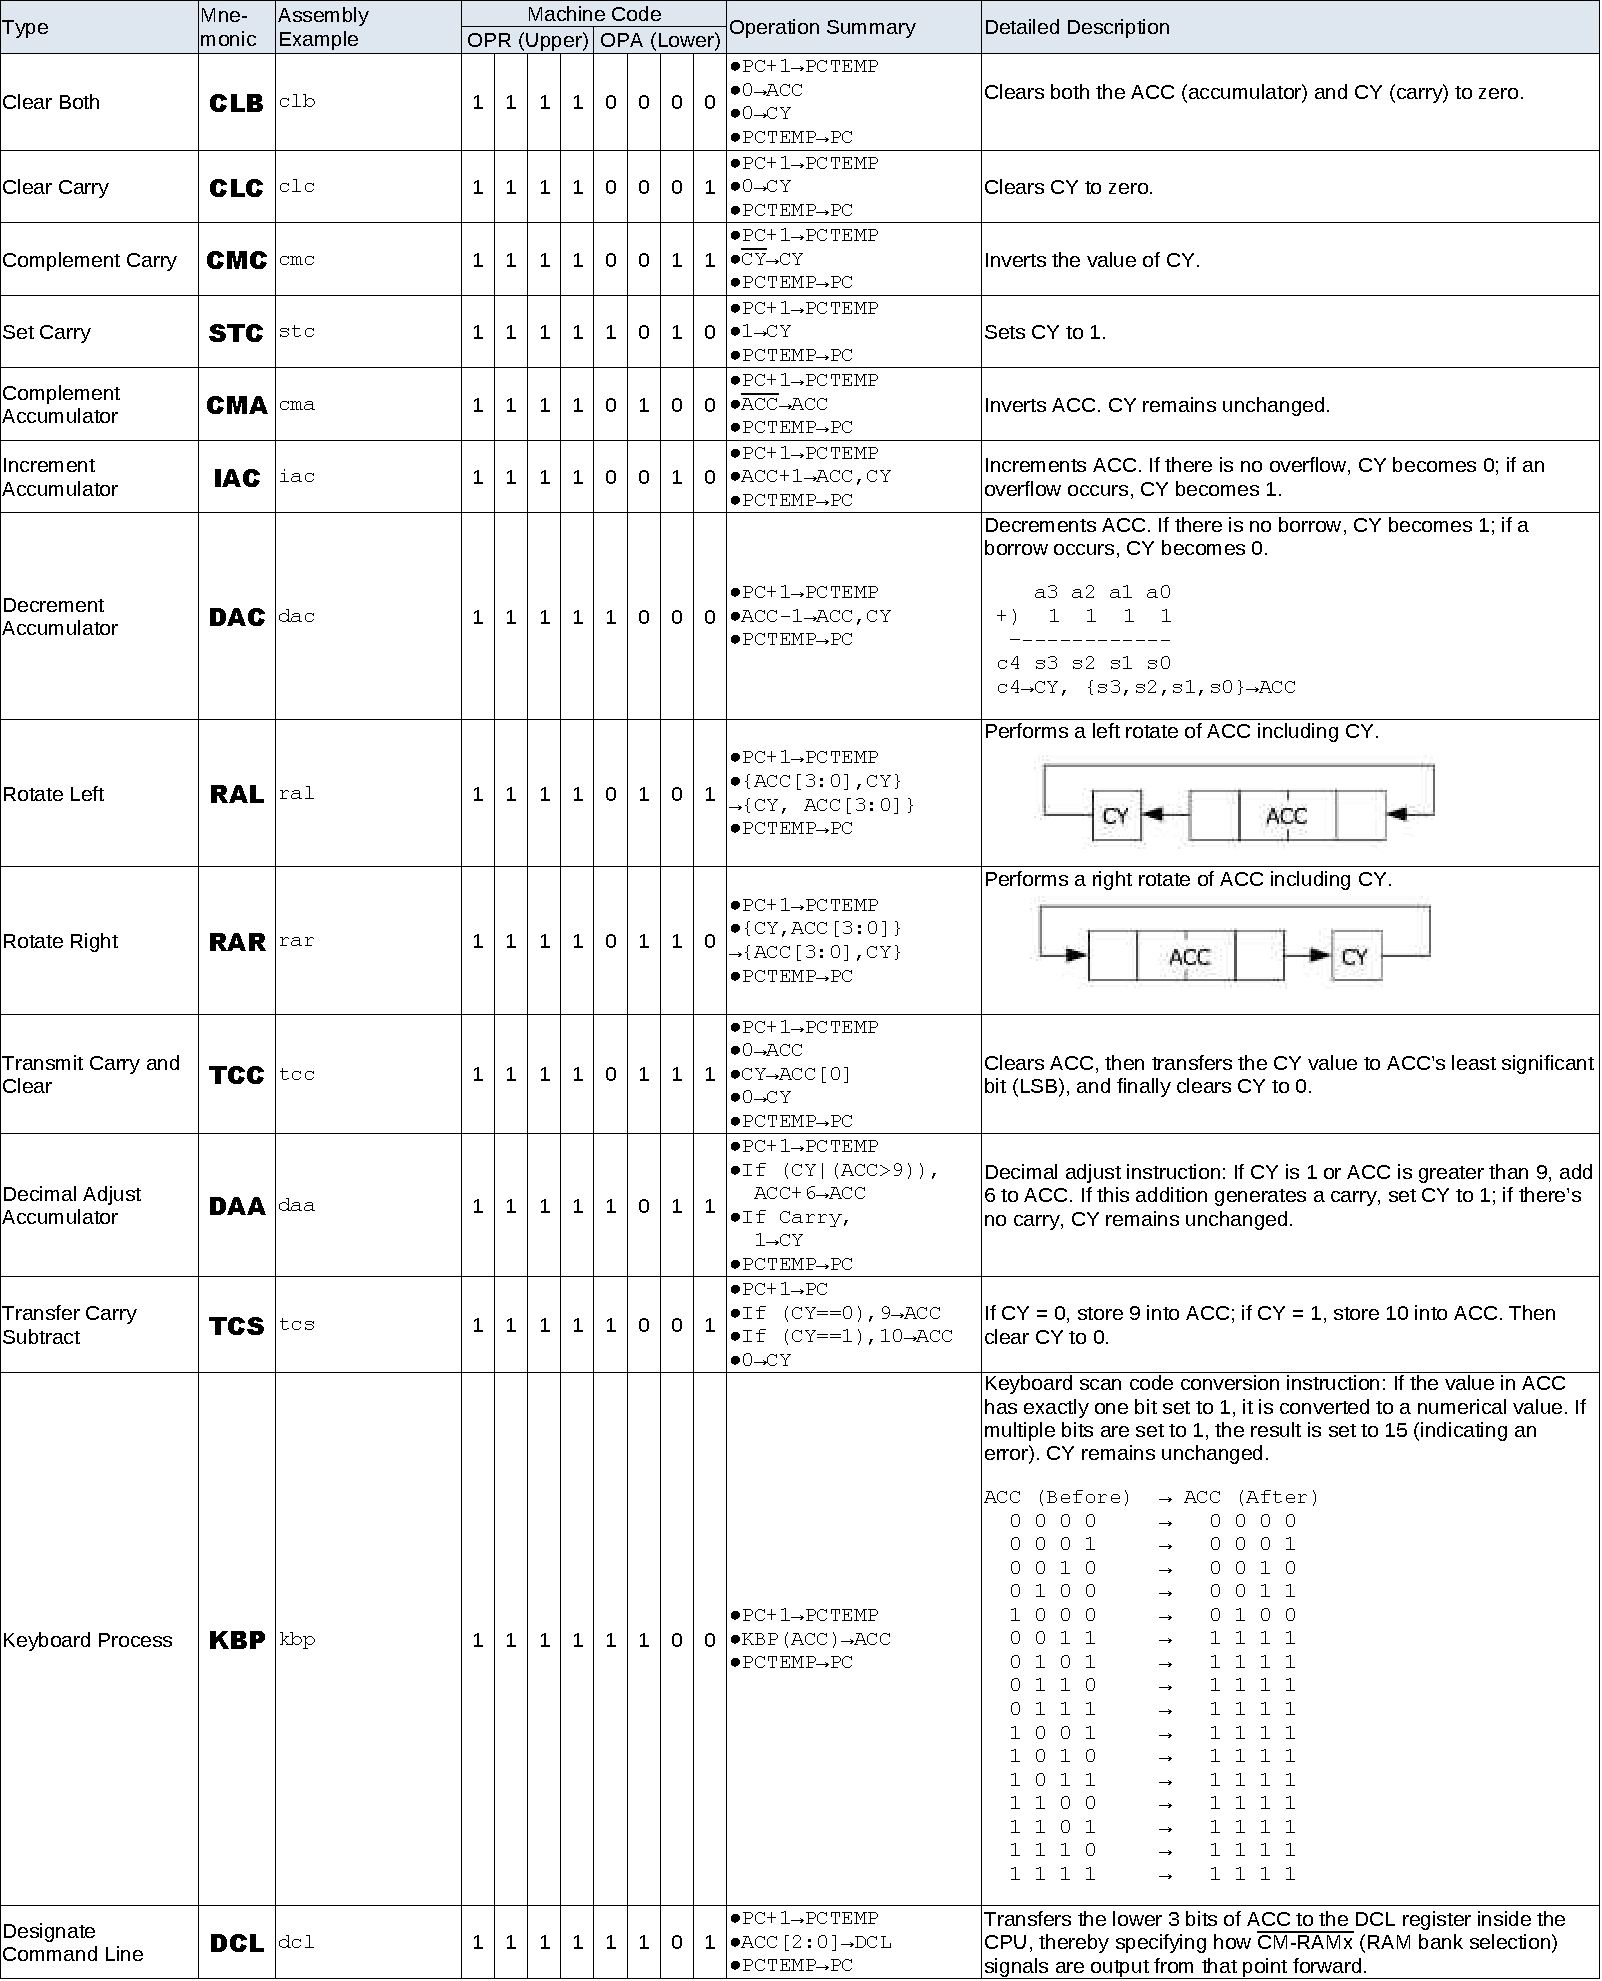
\includegraphics[width=1.00\columnwidth]{./Table/ISA(4)Accumulator.pdf}
    \caption{CPU Instruciton Table (4) : Accumulator}
    \label{tb:ISA4ACCUMULATOR}
\end{table}
%----------------------------------
%==============================================================
\section{Types of Instruction Execution Timing}

Refer again to Figure \ref{fig:CPUINSTRUCTIONTIMING}, which presents all types of instruction execution timing used in the 4004 CPU. Each category is described as follows:

\begin{enumerate}
  \item \textbf{General Type:}  
  Instructions that are executed entirely within the CPU without accessing external data. These are one-word instructions that complete in a single instruction cycle.

  \item \textbf{SRC Type:}  
  The \texttt{SRC} instruction outputs the lower 8 bits of the ROM/RAM address via states X2 and X3. During state X2, $\overline{\text{CM-ROM}}$ and $\overline{\text{CM-RAMx}}$ (selected by the DCL register) are asserted to transfer address information to ROM/RAM. This is a one-word instruction that completes in a single instruction cycle.

  \item \textbf{WR Type (Write):}  
  Instructions that write data to external targets such as ROM output ports, RAM main memory characters, RAM status characters, or RAM output ports. The opcode is fetched in state M2 and interpreted by both CPU and ROM/RAM, requiring assertion of $\overline{\text{CM-ROM}}$ and $\overline{\text{CM-RAMx}}$. Data is written during state X2. One-word, one-cycle execution.

  \item \textbf{RD Type (Read):}  
  Instructions that read data from ROM input ports, RAM main memory characters, or RAM status characters. Like WR instructions, the opcode is fetched in state M2 and interpreted by CPU and ROM/RAM. $\overline{\text{CM-ROM}}$ and $\overline{\text{CM-RAMx}}$ are asserted, and data is read during state X2. One-word, one-cycle execution.

  \item \textbf{FIM Type:}  
  The \texttt{FIM} instruction is a two-word instruction completed in two instruction cycles. The second word, fetched during M1 and M2 of the second cycle, is transferred as immediate data into index register pair RmP.

  \item \textbf{FIN Type:}  
  The \texttt{FIN} instruction is one word long but requires two instruction cycles. After recognition in the first cycle, the second cycle uses A1–A3 and M1–M2 states to read from a ROM address. The retrieved data is stored into index register pair RmP. This instruction reads constant values from ROM.
\end{enumerate}

%==============================================================
\section{Instruction Fetch Operation from ROM}

The detailed behavior of instruction fetch operations from ROM is summarized in Figure \ref{fig:CPUINSTRUCTIONFETCH}. During states A1 and A2, the address signals output from the CPU—specifically PC[3:0] and PC[7:4]—are received by all ROM chips. In state A3, when the $\overline{\text{CM-ROM}}$ signal is asserted, the address signal PC[11:7] is also received by all ROM chips; however, PC[11:8] corresponds to the ROM chip number. This enables selection of the specific ROM chip from which the CPU intends to fetch the instruction.

Following this process, in states M1 and M2, the selected ROM chip outputs the high-order instruction code (OPR) and low-order instruction code (OPA), which the CPU then fetches.

In state A3, the $\overline{\text{CM-ROM}}$ signal is asserted. Although CPU and ROM operate synchronously—so $\overline{\text{CM-ROM}}$ is not strictly necessary—the use of $\overline{\text{CM-ROM}}$ becomes advantageous when expanding the number of connected ROM chips beyond 16. It simplifies the design of external circuits for ROM selection.

Additionally, $\overline{\text{CM-RAMx}}$ is also asserted during state A3. While this has no inherent significance in standard operation, it becomes meaningful if external circuitry has been added to allow ROM access via $\overline{\text{CM-RAMx}}$—for example, when expanding ROM capacity by repurposing RAM access signals.

%----------------------------------
\begin{figure}[htbp]
    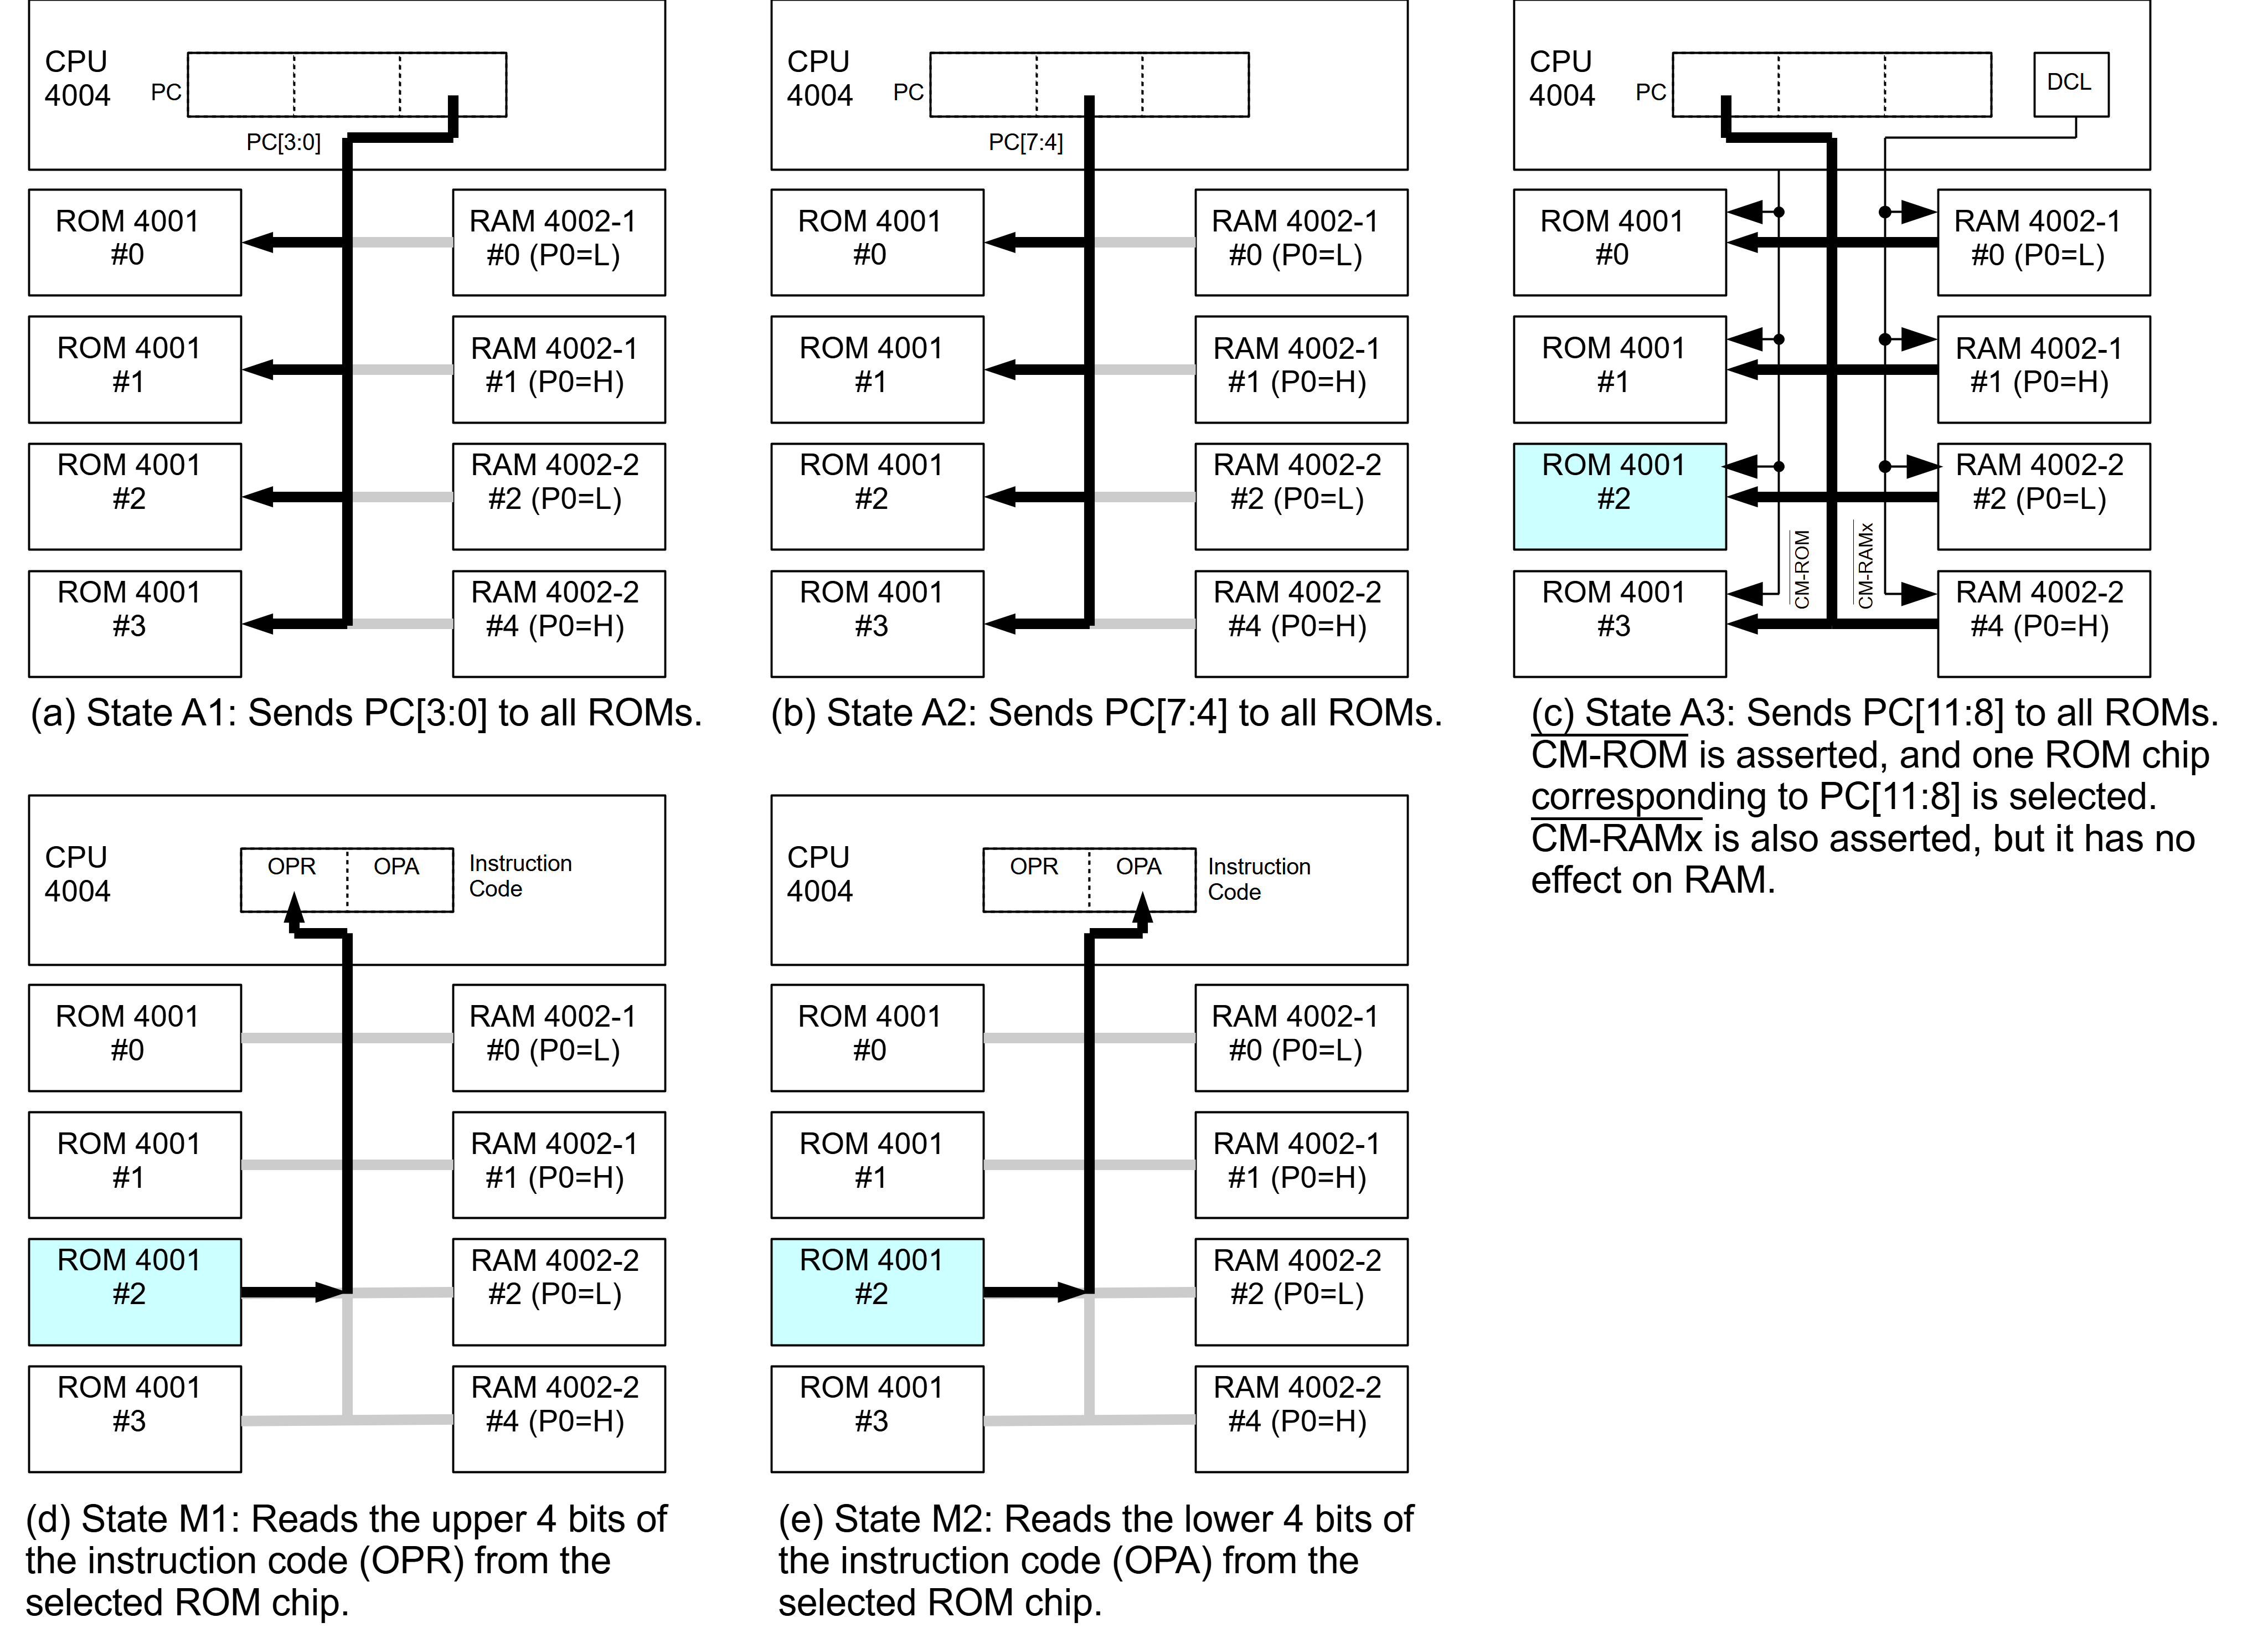
\includegraphics[width=1.0\columnwidth]{./Figure/CPUInstructionFetch.png}
    \caption{4004 CPU Instruction Fetch}
    \label{fig:CPUINSTRUCTIONFETCH}
\end{figure}
%----------------------------------

%==============================================================
\section{CPU Data Read Operation}
The CPU's data read operation for external devices such as RAM main memory characters, RAM status characters, and ROM input ports is illustrated in Figure \ref{fig:CPUINSTRUCTIONREAD}. When accessing external devices, the operation is split into two instructions: one to transmit address information and another to perform the actual data access.

%----------------------------------
\begin{figure}[htbp]
    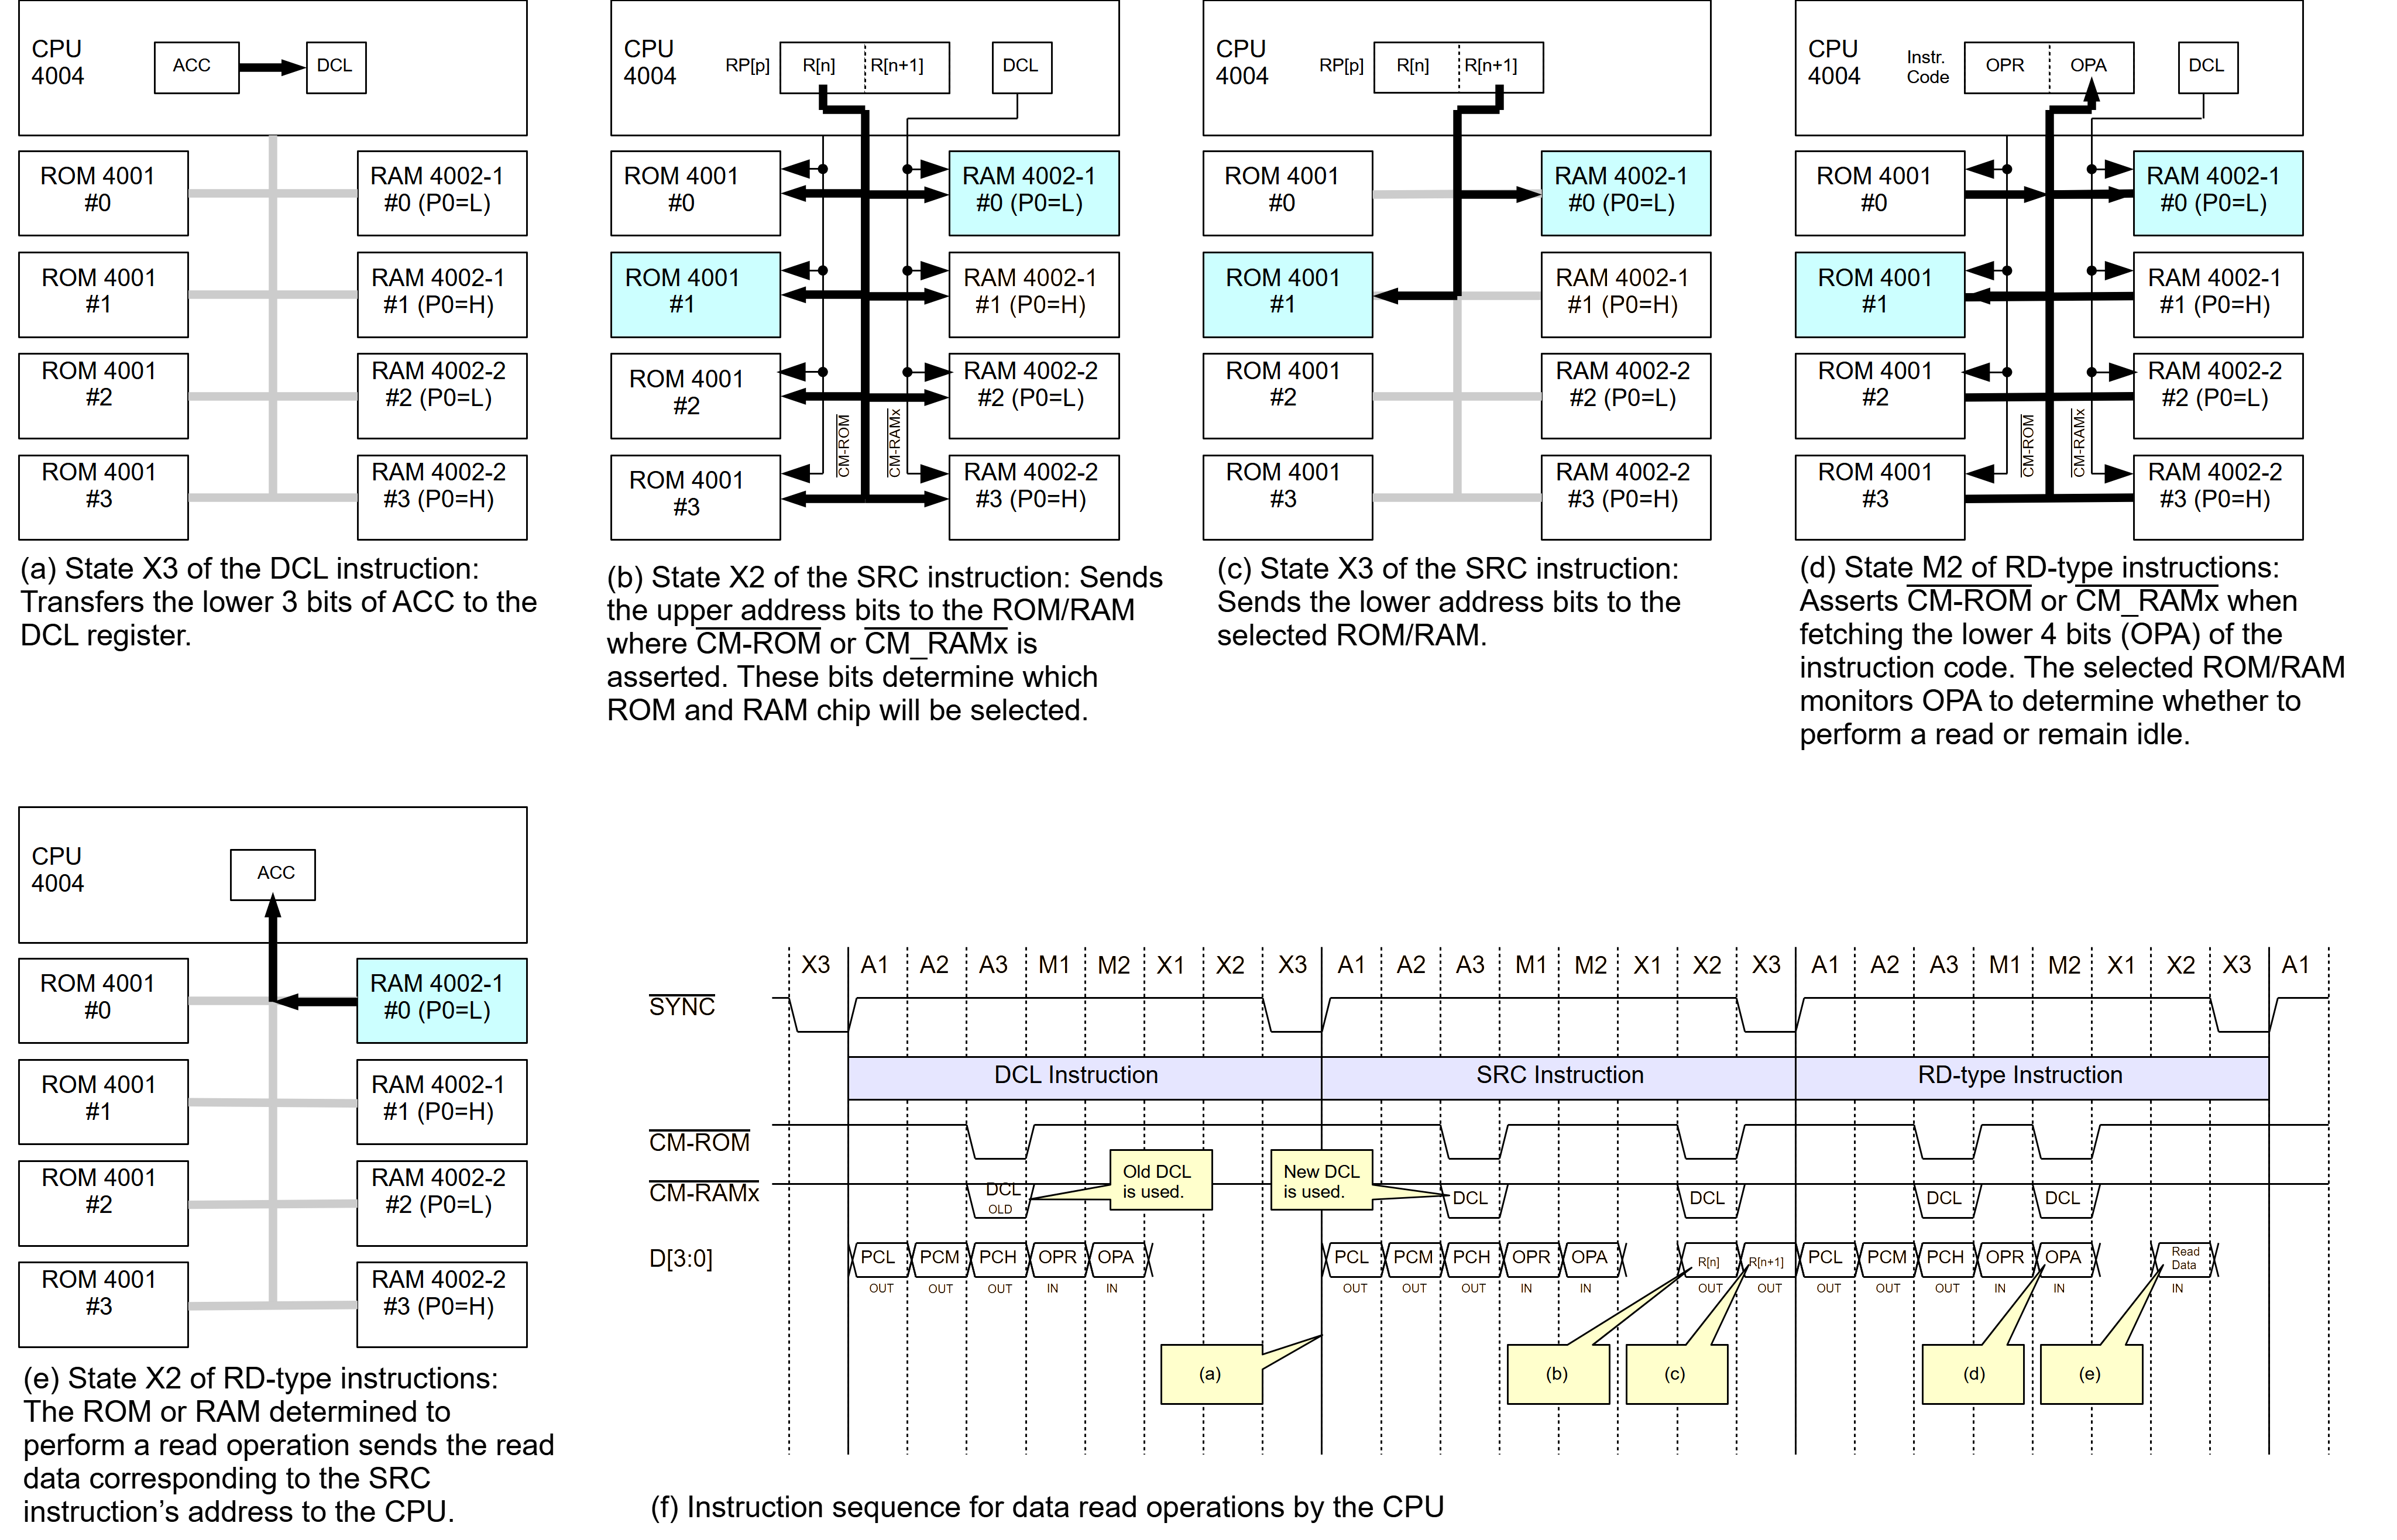
\includegraphics[width=1.0\columnwidth]{./Figure/CPUInstructionRead.png}
    \caption{4004 CPU Data Read Operation}
    \label{fig:CPUINSTRUCTIONREAD}
\end{figure}
%----------------------------------
%----------------------------------
\subsection{DCL Instruction: RAM Bank Selection}
When accessing RAM, the target RAM bank must first be designated by executing the \texttt{DCL} instruction as shown in Figure \ref{fig:CPUINSTRUCTIONREAD}(a). This instruction stores the lower 3 bits of the accumulator into the DCL register. According to the value of DCL, a subsequent instruction will assert the corresponding $\overline{\text{CM-RAMx}}$ signal.

Table[ref{tb:DCLANDCMRAM} shows the correspondence between DCL values and CM-RAMx signals.  
- For systems with up to 4 RAM banks, only four DCL patterns (3'b000, 3'b001, 3'b010, 3'b100) are used to assert $\overline{\text{CM-RAMx}}$ in a one-hot manner, eliminating the need for external circuits.  
- For systems with up to 8 RAM banks, all 8 combinations of the 3-bit DCL are used. Since $\overline{\text{CM-RAMx}}$ may not be one-hot in this case, external decoding circuits (see Figure \ref{fig:DCLDECODER}) are used to expand the number of $\overline{\text{CM-RAMx}}$ lines.

If RAM is not being accessed, or the same bank is reused, or the default DCL value (3'b000) is retained, executing the DCL instruction is unnecessary.

%----------------------------------
\begin{table}[htbp]
    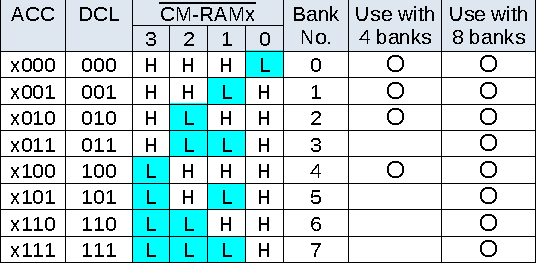
\includegraphics[width=0.5\columnwidth]{./Table/DCLandCMRAM.pdf}
    \caption{Correspondence between DCL values and $\overline{\text{CM-RAMx}}$ signals}
    \label{tb:DCLANDCMRAM}
\end{table}
%----------------------------------
%----------------------------------
\begin{figure}[htbp]
    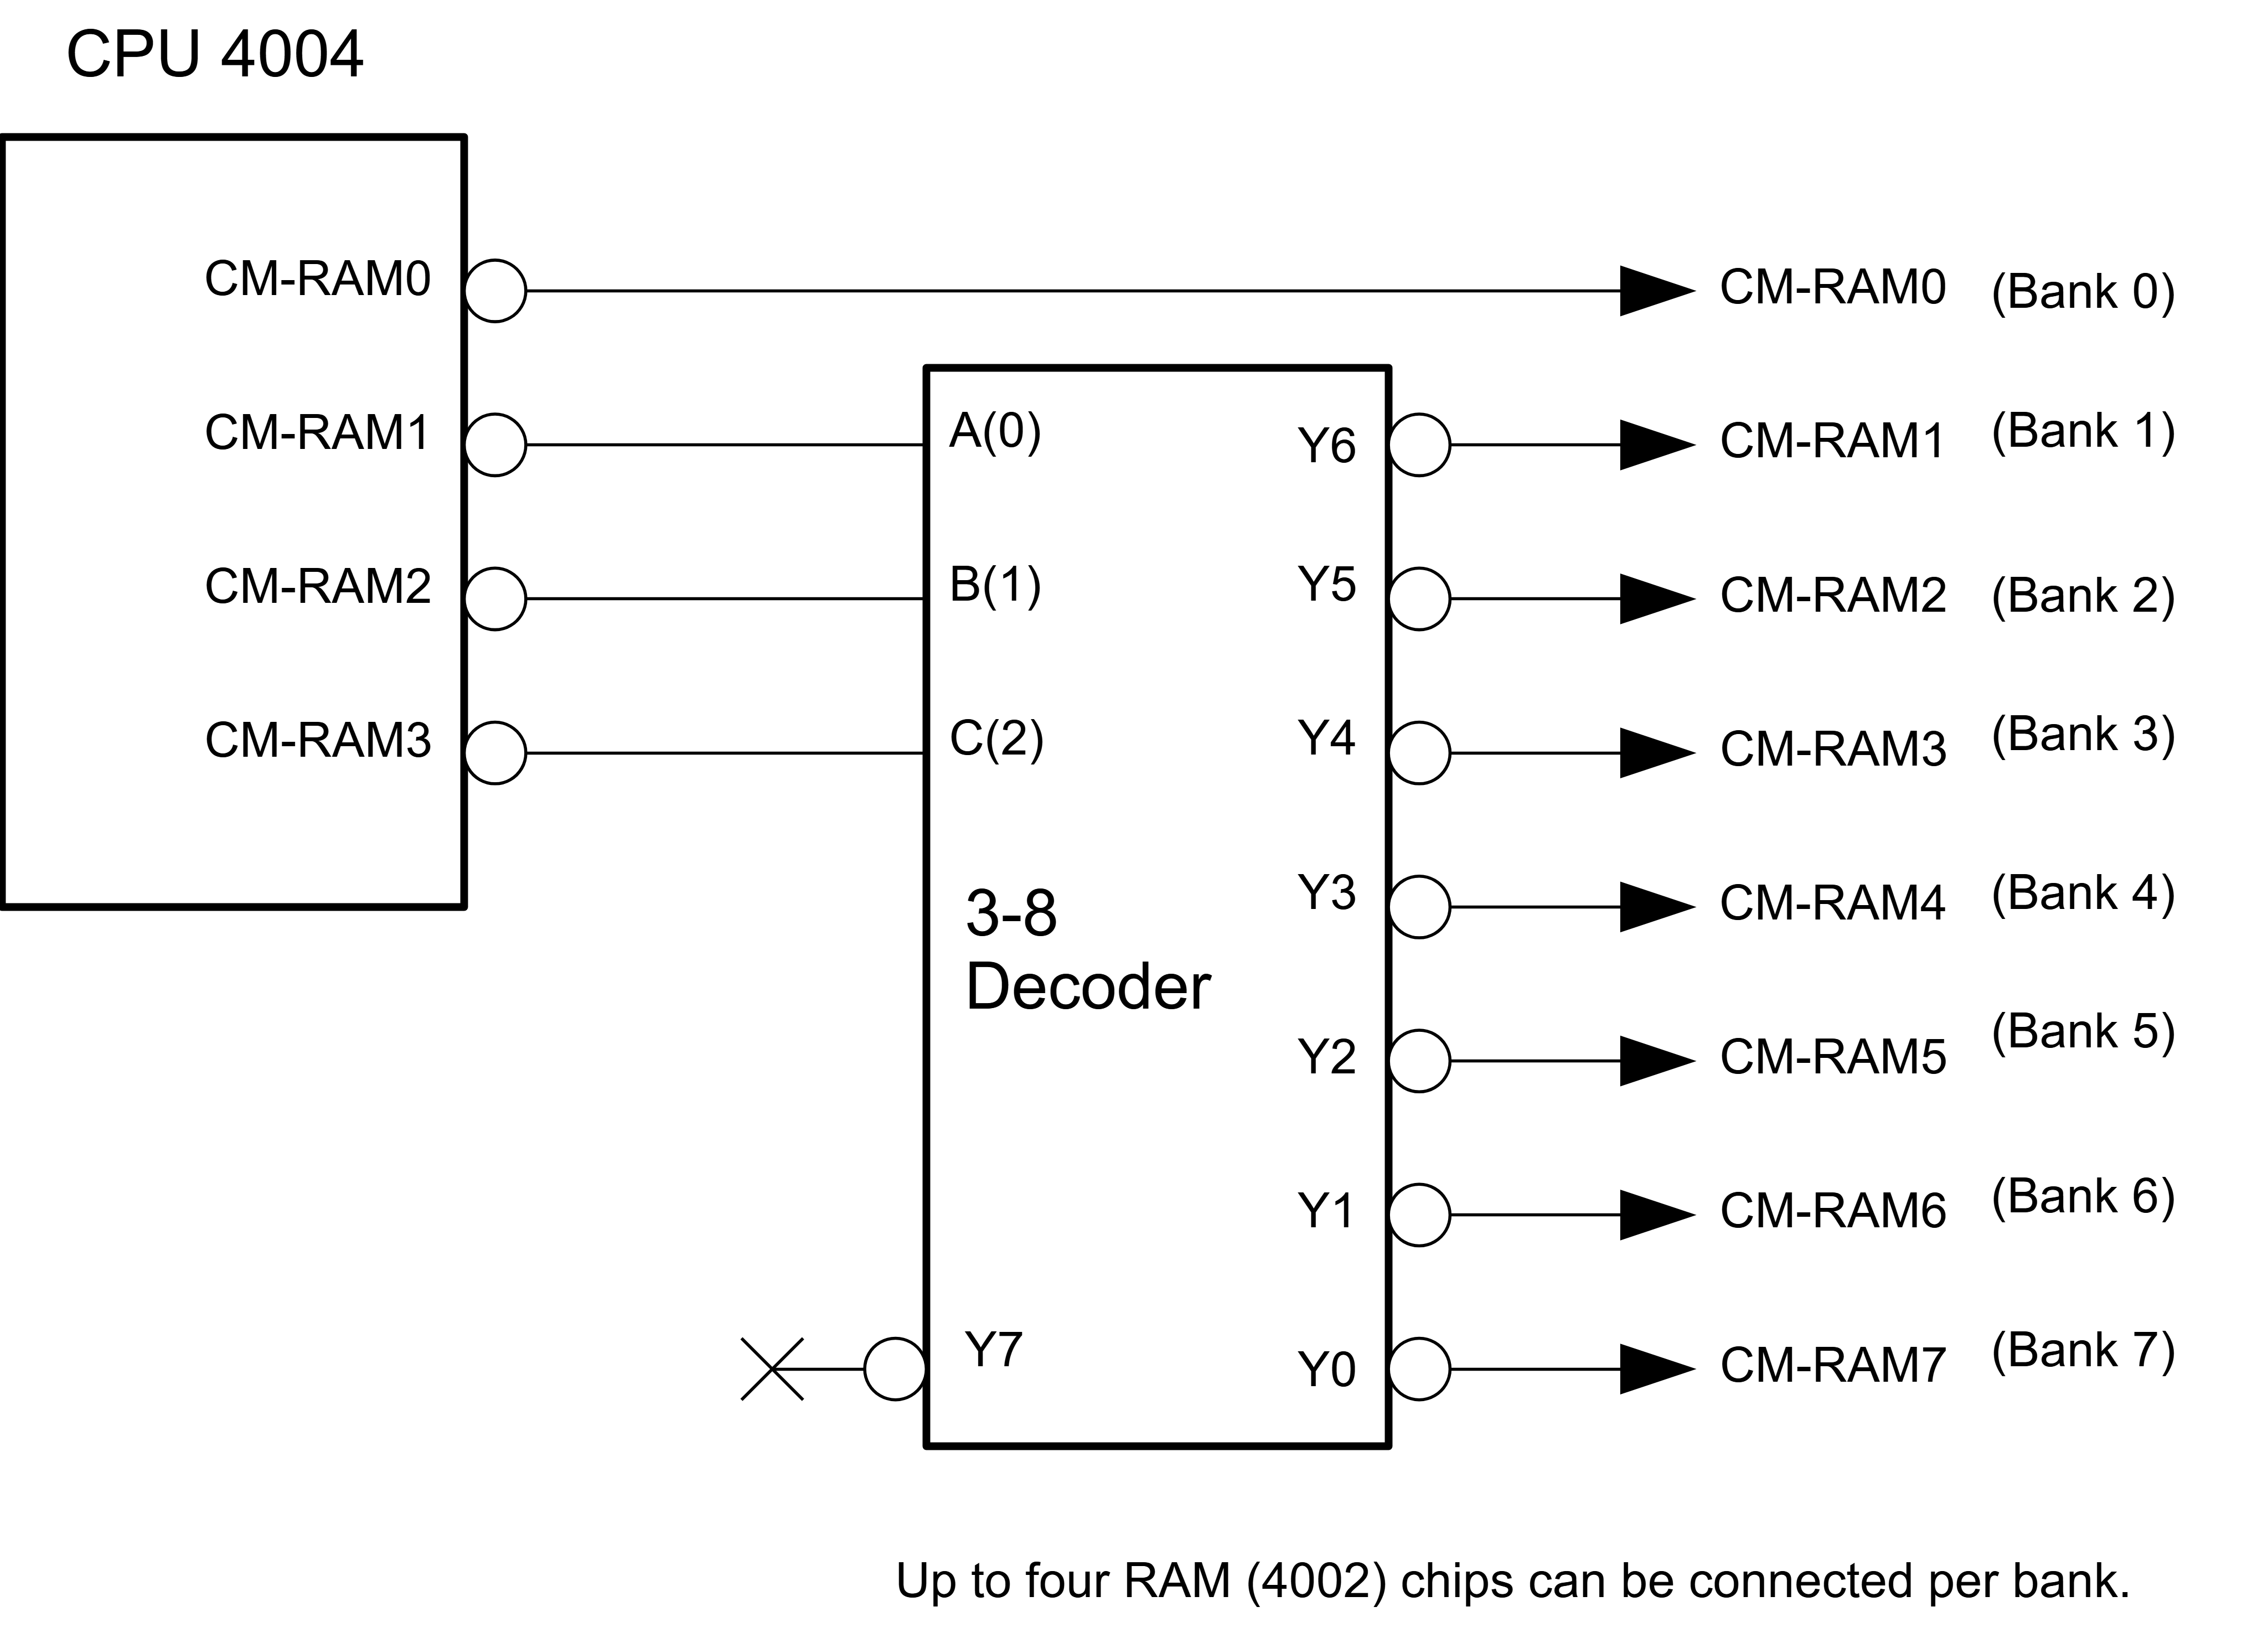
\includegraphics[width=0.5\columnwidth]{./Figure/DCLDecoder.png}
    \caption{RAM Bank Expansion and DCL Decoder}
    \textit{To increase the number of CM-RAM lines. Up to 4 RAM (4002) chips can be connected per bank.}
    \label{fig:DCLDECODER}
\end{figure}
%----------------------------------

%----------------------------------
\subsection{SRC Instruction: Address Transmission}
Next, the \texttt{SRC} instruction is executed as shown in Figures \ref{fig:CPUINSTRUCTIONREAD}(b) and (c). The instruction transfers the 8-bit value stored in index register pair RnP to ROM/RAM as address information. The address structure is summarized in Table \ref{tb:SRCADDRESSSTRUCTURE}.

- In state X2, CM-ROM and CM-RAMx are asserted. The upper 4 bits of the address are transmitted to all ROM chips and to RAM chips within the bank selected by CM-RAMx. As shown in Table~4, this portion contains chip select information. Once the ROM/RAM receives the upper 4 bits, the active ROM and RAM chips are determined.
- In state X3, the lower 4 bits of the address are sent. The ROM/RAM chips activated in state X2 receive this part and await subsequent data access instructions.

Note: The address stored inside the ROM/RAM chip by the SRC instruction is retained even after the data access instruction is executed. Thus, when accessing the same location again, the SRC instruction does not need to be re-executed.

The SRC address for RAM main memory characters is calculated as:  
\texttt{(Chip \# $\times$ 64) + (Register \# $\times$ 16) + (Character \#)}

%----------------------------------
\begin{table}[htbp]
    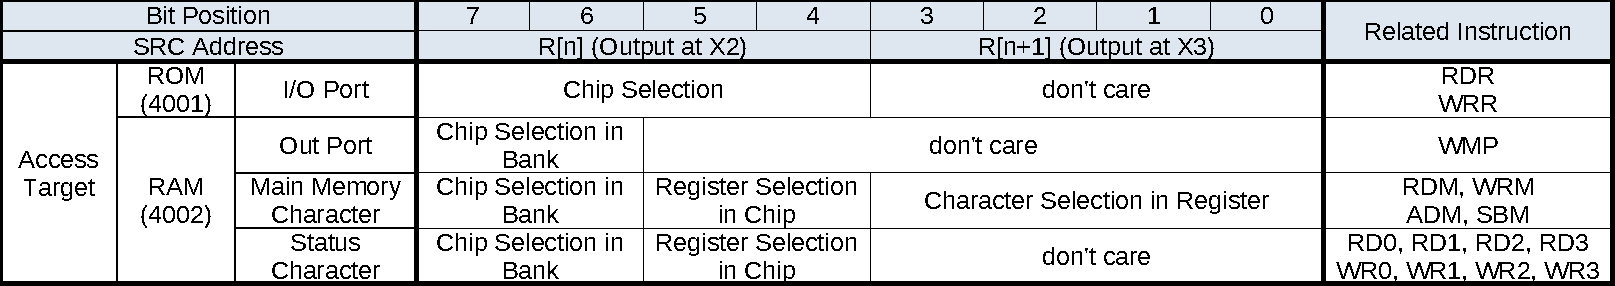
\includegraphics[width=1.00\columnwidth]{./Table/SRCAddressStructure.pdf}
    \caption{SRC Address Structure}
    \label{tb:SRCADDRESSSTRUCTURE}
\end{table}
%----------------------------------

%----------------------------------
\subsection{Data Access Instructions}
To perform actual data read/write operations, a data access instruction is executed. These instructions all have an opcode upper 4 bits (OPR) equal to 4'b1110, allowing the CPU to recognize them as data access instructions when fetched in state M1.

Then, during state M2—when the lower 4 bits of the opcode (OPA) are fetched—$\overline{\text{CM-ROM}}$ and the $\overline{\text{CM-RAMx}}$ signal corresponding to the DCL register are asserted, as shown in Figures \ref{fig:CPUINSTRUCTIONREAD}(d).

During this M2 state, ROM/RAM interprets the OPA on the data bus to determine the type of access (read or write) and the target.  
If the instruction performs a read operation, the ROM/RAM outputs the data to the data bus in state X2 (same instruction cycle), as illustrated in Figures \ref{fig:CPUINSTRUCTIONREAD}(e), and the CPU stores the data into the accumulator.

Refer to Table \ref{tb:ISA3DATAACCESS} for types of data read instructions.

%==============================================================
\section{CPU Data Write Operation}

Figure \ref{fig:CPUINSTRUCTIONWRITE} illustrates the sequence of operations when the CPU writes to external components such as RAM main memory characters, RAM status characters, or output ports of ROM/RAM. The write operation follows a sequence fundamentally similar to that of a read.

During state X2 of the data access instruction, the CPU outputs the write data—stored in the accumulator—onto the data bus. The target ROM or RAM component, having been selected by prior addressing signals, receives this data and writes it to the designated address.

Refer to Table \ref{tb:ISA3DATAACCESS} for the types of data write instructions available.
%----------------------------------
\begin{figure}[htbp]
    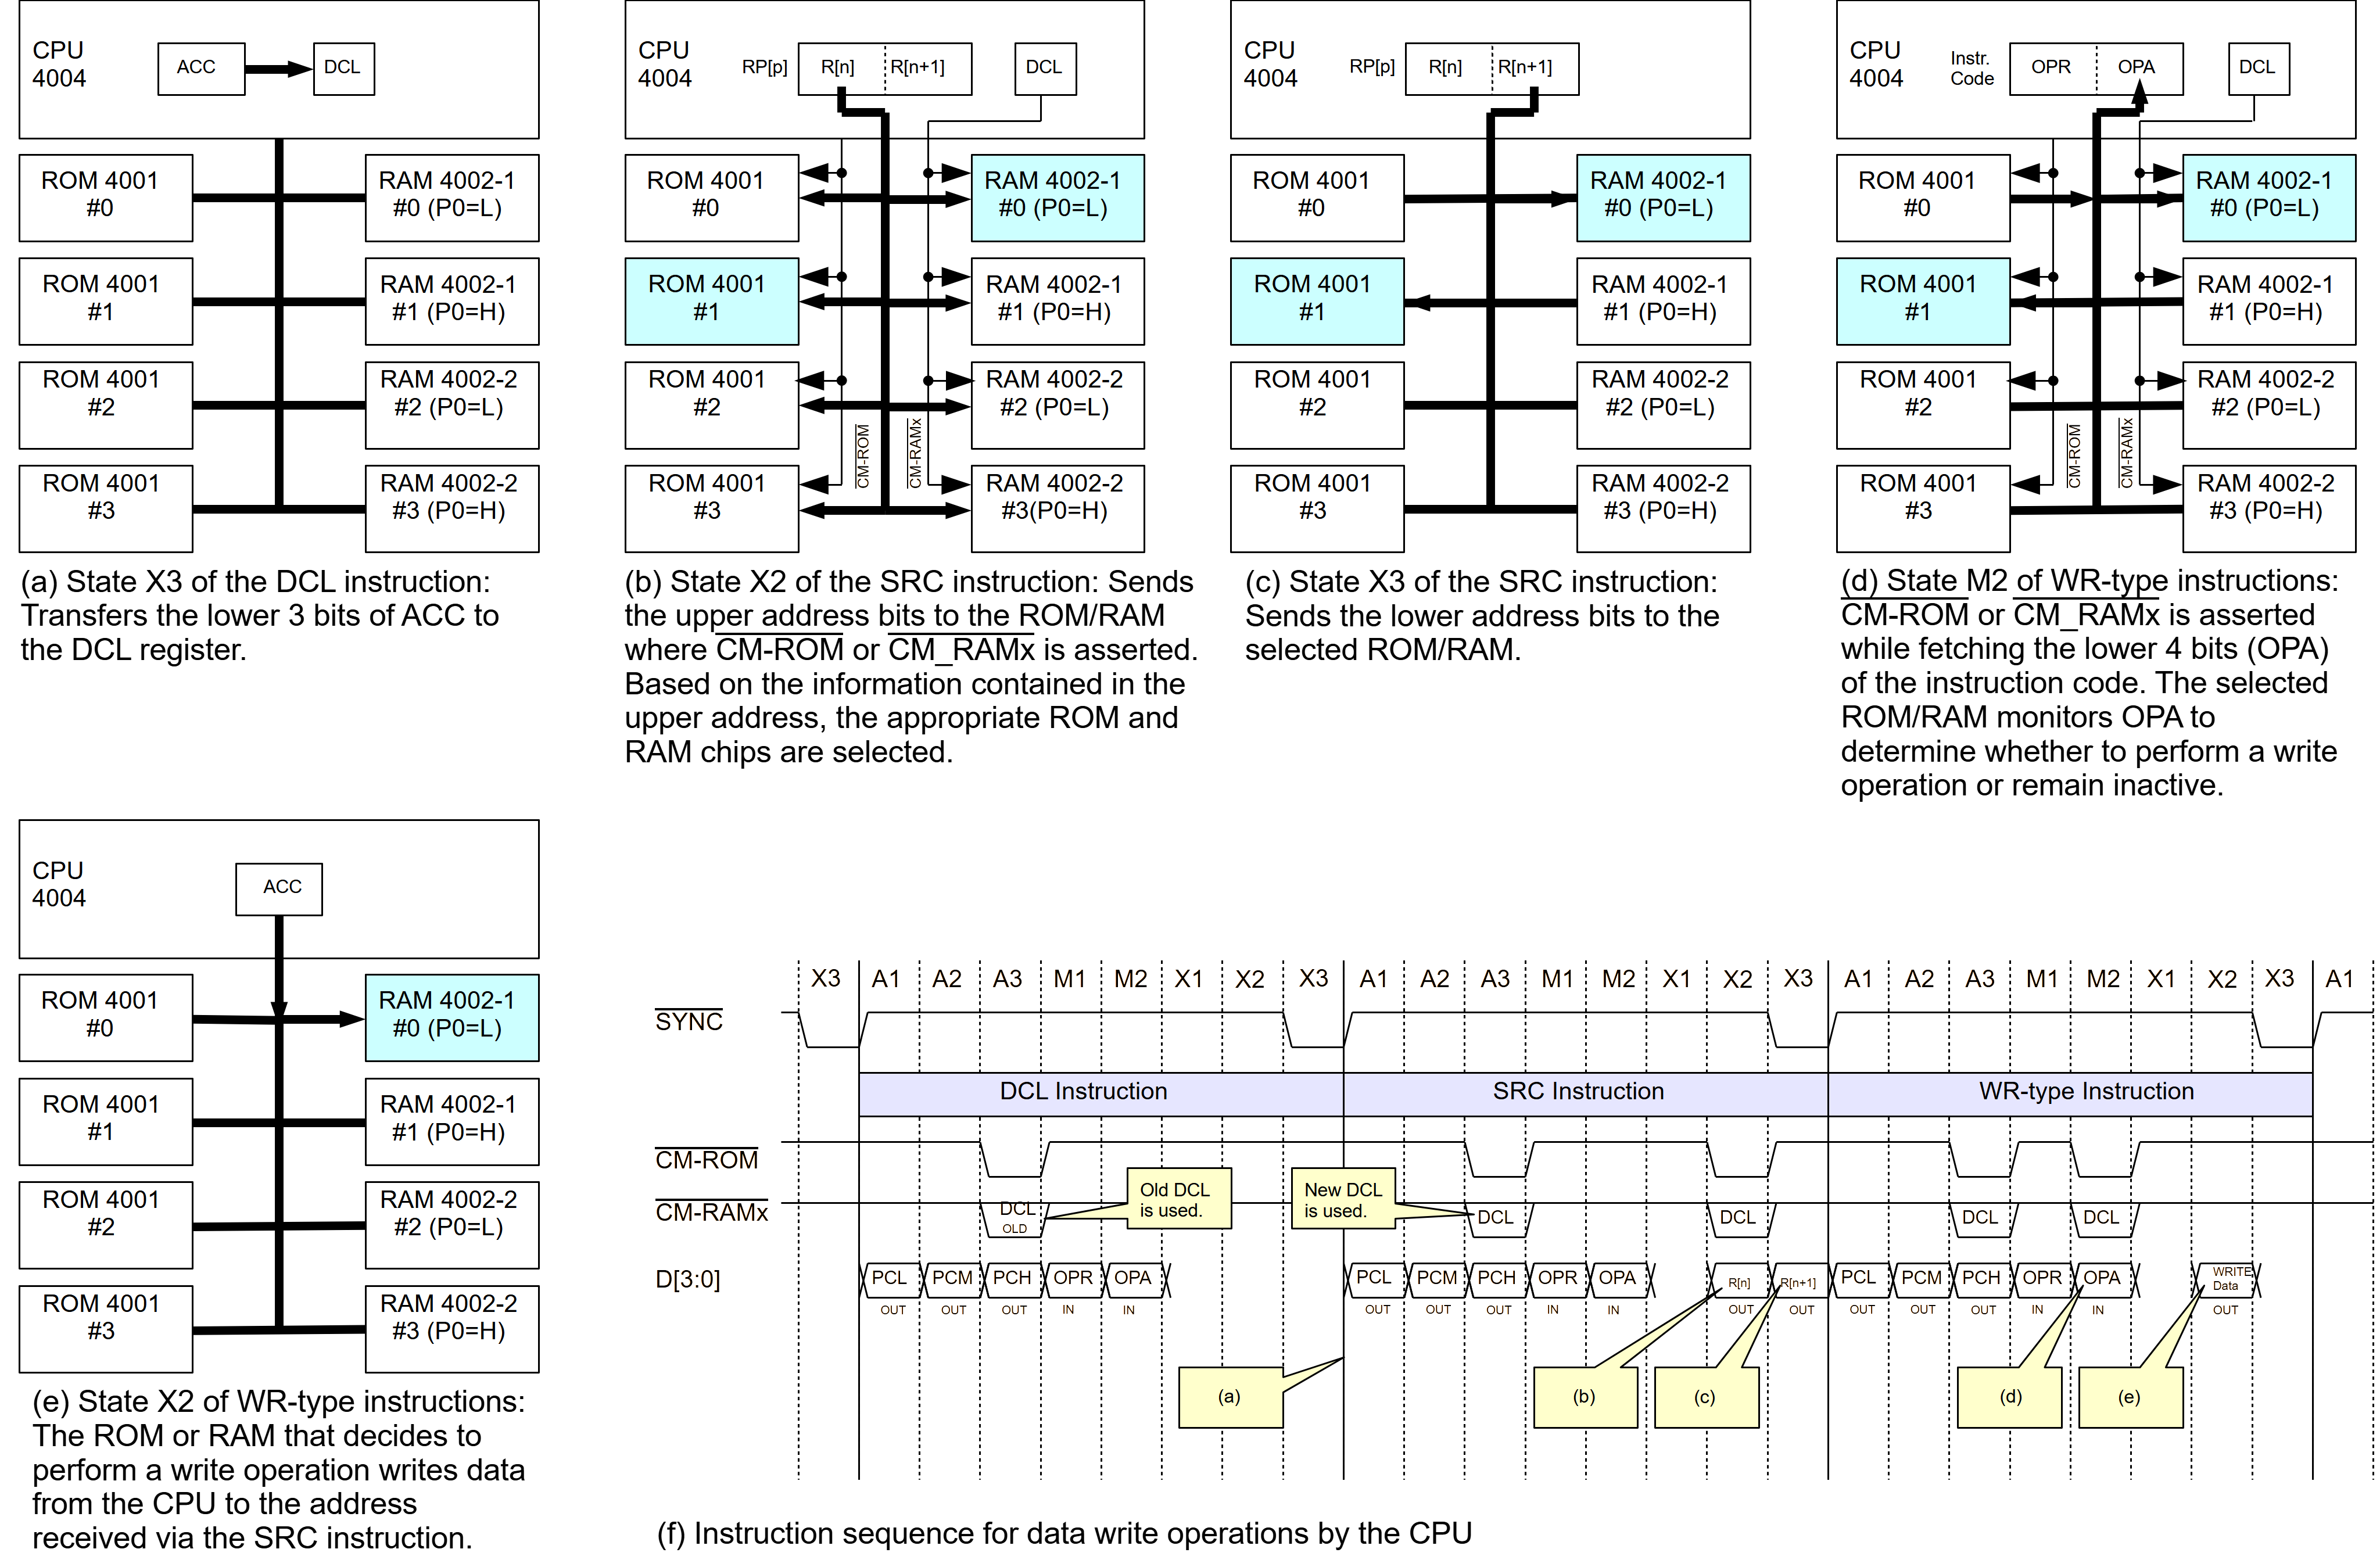
\includegraphics[width=1.0\columnwidth]{./Figure/CPUInstructionWrite.png}
    \caption{4004 CPU Data Write Operation}
    \label{fig:CPUINSTRUCTIONWRITE}
\end{figure}
%----------------------------------

%==============================================================
\section{Subroutine Call Operation in the 4004 CPU}
Modern CPUs typically handle subroutine calls by saving the return address to a stack located in memory space. In contrast, the 4004 CPU employs a dedicated stack mechanism, consisting of four levels of 12-bit program address registers, to implement subroutine calls. This structure is illustrated in Figure \ref{fig:CPUPROGRAMMERSMODEL}.

Figure \ref{fig:CPUSUBROUTINECALL} outlines the operational behavior:

\begin{itemize}
  \item \textbf{(a)} Initially, the program address register pointed to by the stack pointer (SP) serves as the program counter (PC).
  
  \item \textbf{(b)} When a subroutine call instruction (\texttt{JMS}) is executed, the SP is incremented, and the target address of the subroutine is stored in the newly selected program address register, which then functions as the new PC. Meanwhile, the previously selected register (prior to SP increment) retains the return address—the address of the instruction immediately following the \texttt{JMS} call.
  
  \item \textbf{(c, d)} Repeated executions of \texttt{JMS} result in the same behavior, each time nesting one level deeper in the stack.
  
  \item \textbf{(e)} Since the stack has only four levels, executing \texttt{JMS} four times consecutively will overwrite the earliest return address. Therefore, the 4004 CPU imposes a limit of three subroutine nesting levels.
  
  \item \textbf{(f)} When a subroutine return instruction (\texttt{BBL}) is executed, the SP is decremented, and the program address register that now contains the previous return address becomes the new PC, allowing instruction execution to resume at the correct return point.
\end{itemize}

%----------------------------------
\begin{figure}[htbp]
    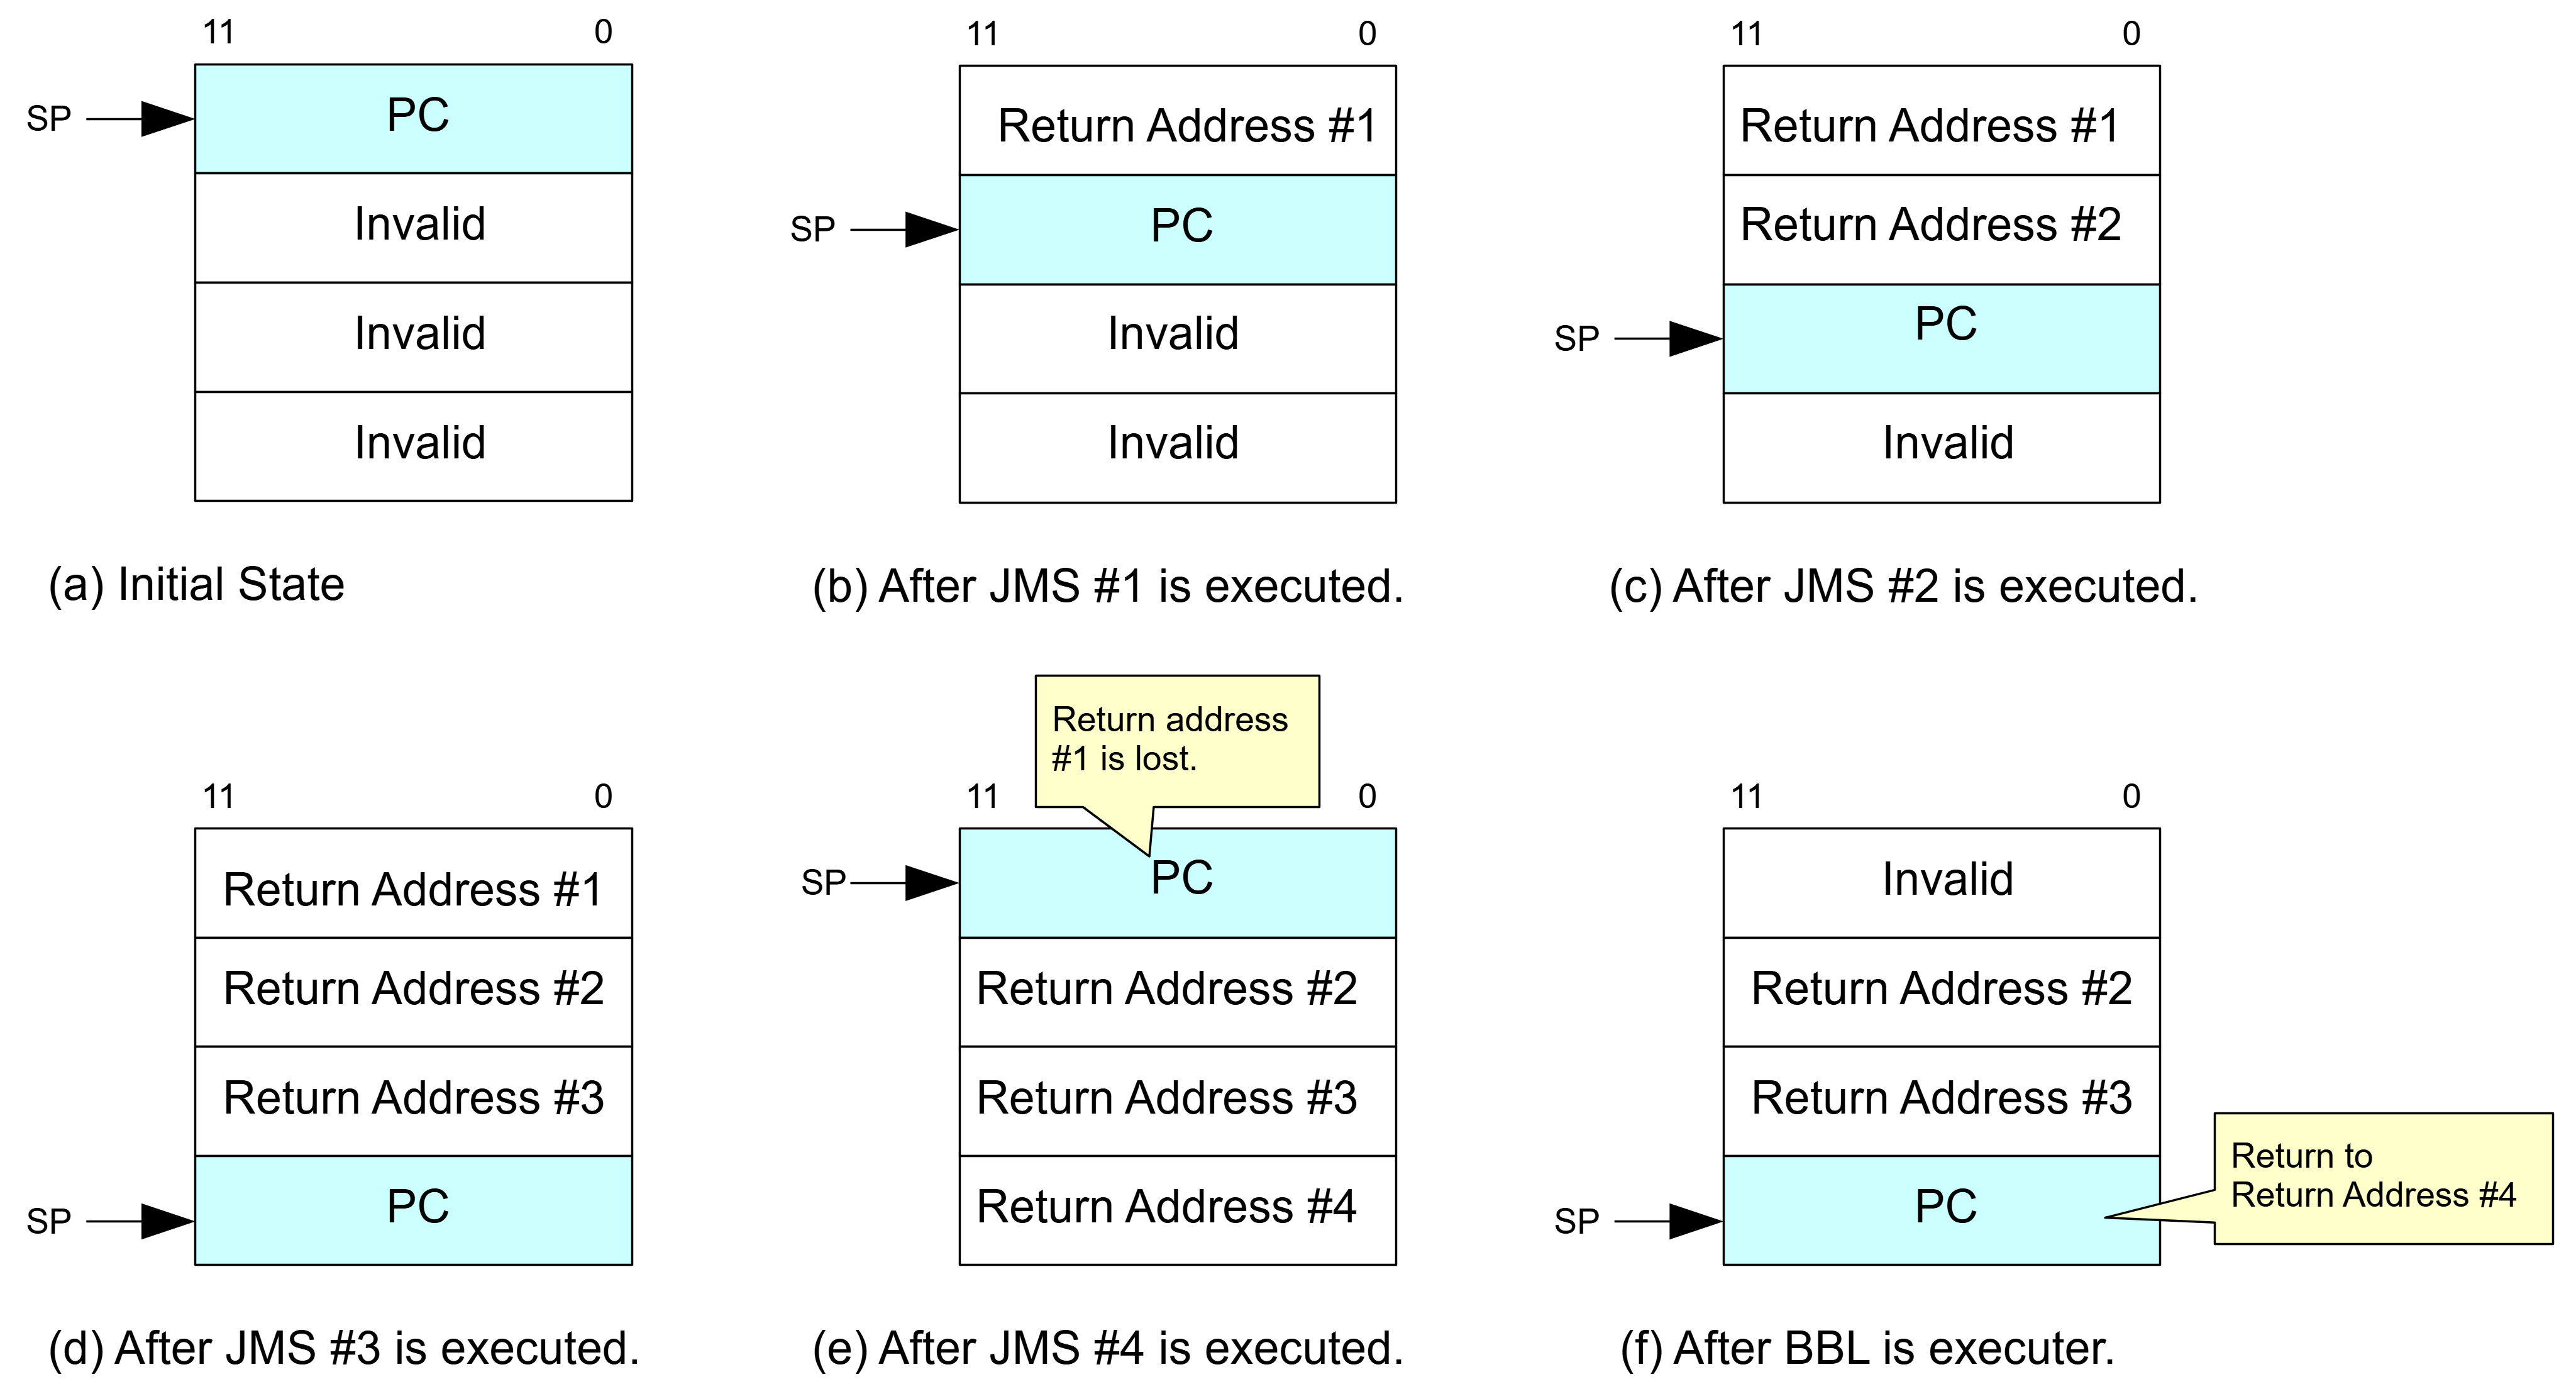
\includegraphics[width=1.0\columnwidth]{./Figure/CPUSubroutineCall.png}
    \caption{4004 CPU Subroutine Call}
    \label{fig:CPUSUBROUTINECALL}
\end{figure}
%----------------------------------

%==============================================================
\section{TEST Pin as an Alternative to Interrupts}
Unlike modern CPUs that naturally support interrupt handling, the 4004 CPU does not have a built-in interrupt feature. However, it does provide a mechanism that can function similarly to an interrupt: the \texttt{TEST} input pin.

The TEST signal can be included as part of the conditional branching logic within the \texttt{JCN} (Jump Conditional) instruction. By monitoring the input level of the TEST pin and executing \texttt{JCN} instructions at regular intervals, the system can respond to external conditions with a limited latency. Thus, the TEST pin can effectively serve as an interrupt trigger.

%==============================================================
\section{Instructions Located at ROM Page Boundaries}
For one-word instructions that modify only the lower 8 bits of the PC (program counter), if such instructions reside at the final address of a 256-byte ROM page (\texttt{0x..FF}), they will branch to an address within the next page. This is because the system generates \texttt{PC+1} and then replaces only the lower 8 bits for the branch.

Similarly, for two-word instructions that modify only the lower 8 bits of the PC, if they are located at the final address or its immediate predecessor (\texttt{0x..FF} or \texttt{0x..FE}), they will also branch into the next ROM page. In this case, the system generates \texttt{PC+2} and updates only the lower 8 bits of the PC for branching.

%==============================================================
\section{Timing of PC Update}
From these observations, the timing for PC updates has been interpreted and incorporated into the next chapter's RTL design as follows:

Whether the instruction is one-word or two-word, the address for the next instruction cycle (\texttt{PC+1}) is stored in a temporary signal named \texttt{PCTEMP} at the beginning of state A1. Any references to PC during instruction execution refer to \texttt{PCTEMP}.

For non-branching instructions or conditional branches that do not result in a branch, \texttt{PCTEMP} is transferred to \texttt{PC} during the final state X3 of the instruction cycle.

If a branch occurs, the final state X3 updates \texttt{PC} with the branch destination address. In cases where only the lower 8 bits of the PC are modified, the upper 4 bits \texttt{PC[11:8]} are assigned from \texttt{PCTEMP[11:8]}.

%==============================================================
\section{FIN Instruction and ROM Page Boundaries}
The \texttt{FIN} instruction is unique in that although it is a one-word instruction, it spans two instruction cycles and requires careful handling of PC updates.

If a FIN instruction resides at the last address of a ROM page (\texttt{0x..FF}), it fetches data from the next page. At the beginning of the first cycle, \texttt{PC+1} is stored in \texttt{PCTEMP}, but no transfer to \texttt{PC} occurs at the end of X3.

During the second instruction cycle, states A1 to A3 output the ROM read address:  
- A1 outputs \texttt{R0P[3:0]}  
- A2 outputs \texttt{R0P[7:4]}  
- A3 outputs \texttt{PCTEMP[11:7]}

Finally, PC is updated with the value of \texttt{PCTEMP} during the last X3 state of the second cycle.

%==============================================================
\section{Appreciating the Wisdom of the Pioneers}
%----------------------------------
\subsection{Ingenuity in Packing Maximum Functionality into Minimal Hardware}
As we have seen, the MCS-4 system is filled with ingenious techniques for extracting the maximum functionality from minimal hardware. Each chip is housed in a compact 16-pin package, and address and data are transmitted time-divisionally over a 4-bit data bus. Through tightly coordinated operation of the CPU, ROM, and RAM, interface signals are minimized, enabling the construction of a microcomputer system with simple interconnections. One striking revelation is that instruction decoding is not limited to the CPU—the ROM and RAM also participate in it.

%----------------------------------
\subsection{Characteristics Resembling Modern RISC Architectures}
The CPU’s index register group, R0–R15, provides numerous registers for temporary data storage within the CPU itself. This reduces reliance on memory access, which can degrade performance—an idea remarkably similar to the general-purpose registers used in modern RISC (Reduced Instruction Set Computer) architectures. Quite fascinating, isn’t it?

%----------------------------------
\subsection{Learning from the Wisdom of the Past}
In this way, the MCS-4 demonstrates a remarkably well-crafted architecture for a microcontroller. Its approach to hardware simplification offers valuable insights that can be applied to the design of future embedded systems. Studying it is genuinely enriching.

%==============================================================
